%% 
%% Copyright 2007-2024 Elsevier Ltd
%% 
%% This file is part of the 'Elsarticle Bundle'.
%% ---------------------------------------------
%% 
%% It may be distributed under the conditions of the LaTeX Project Public
%% License, either version 1.3 of this license or (at your option) any
%% later version.  The latest version of this license is in
%%    http://www.latex-project.org/lppl.txt
%% and version 1.3 or later is part of all distributions of LaTeX
%% version 1999/12/01 or later.
%% 
%% The list of all files belonging to the 'Elsarticle Bundle' is
%% given in the file `manifest.txt'.
%% 
%% Template article for Elsevier's document class `elsarticle'
%% with harvard style bibliographic references

\documentclass[preprint,12pt,authoryear]{elsarticle}

%% Use the option review to obtain double line spacing
%% \documentclass[authoryear,preprint,review,12pt]{elsarticle}

%% Use the options 1p,twocolumn; 3p; 3p,twocolumn; 5p; or 5p,twocolumn
%% for a journal layout:
%% \documentclass[final,1p,times,authoryear]{elsarticle}
%% \documentclass[final,1p,times,twocolumn,authoryear]{elsarticle}
%% \documentclass[final,3p,times,authoryear]{elsarticle}
%% \documentclass[final,3p,times,twocolumn,authoryear]{elsarticle}
%% \documentclass[final,5p,times,authoryear]{elsarticle}
%% \documentclass[final,5p,times,twocolumn,authoryear]{elsarticle}

%% For including figures, graphicx.sty has been loaded in
%% elsarticle.cls. If you prefer to use the old commands
%% please give \usepackage{epsfig}

%% The amssymb package provides various useful mathematical symbols
% \usepackage{amssymb}
%% The amsmath package provides various useful equation environments.
% \usepackage{amsmath}
\usepackage{amsmath,amsthm,amssymb,scrextend,mathtools}
\usepackage{hyperref}
\usepackage{newtxmath} %for making indicator function
% \RequirePackage[colorlinks,citecolor=blue,urlcolor=blue,backref=page,backref=page]{hyperref}
%% The amsthm package provides extended theorem environments
%% \usepackage{amsthm}

%% The lineno packages adds line numbers. Start line numbering with
%% \begin{linenumbers}, end it with \end{linenumbers}. Or switch it on
%% for the whole article with \linenumbers.
%% \usepackage{lineno}

\newtheorem{theorem}{Theorem}
\newtheorem{lemma}{Lemma}
\newtheorem{definition}{Definition}
\usepackage{natbib}

\journal{Computational Statistics and Data Analysis}

\begin{document}

\begin{frontmatter}

%% Title, authors and addresses

%% use the tnoteref command within \title for footnotes;
%% use the tnotetext command for theassociated footnote;
%% use the fnref command within \author or \affiliation for footnotes;
%% use the fntext command for theassociated footnote;
%% use the corref command within \author for corresponding author footnotes;
%% use the cortext command for theassociated footnote;
%% use the ead command for the email address,
%% and the form \ead[url] for the home page:
%% \title{Title\tnoteref{label1}}
%% \tnotetext[label1]{}
%% \author{Name\corref{cor1}\fnref{label2}}
%% \ead{email address}
%% \ead[url]{home page}
%% \fntext[label2]{}
%% \cortext[cor1]{}
%% \affiliation{organization={},
%%            addressline={}, 
%%            city={},
%%            postcode={}, 
%%            state={},
%%            country={}}
%% \fntext[label3]{}

\title{Quantile Forecast Matching with a Bayesian Quantile Gaussian Process Model} %% Article title

%% use optional labels to link authors explicitly to addresses:
%% \author[label1,label2]{}
%% \affiliation[label1]{organization={},
%%             addressline={},
%%             city={},
%%             postcode={},
%%             state={},
%%             country={}}
%%
%% \affiliation[label2]{organization={},
%%             addressline={},
%%             city={},
%%             postcode={},
%%             state={},
%%             country={}}

\author[label1]{Spencer Wadsworth} %% Author name
\author[label1]{Jarad Niemi}

%% Author affiliation
\affiliation[label1]{organization={Iowa State Univerity, Department of Statistics},%Department and Organization
            addressline={2438 Osborn Dr}, 
            city={Ames},
            postcode={50011}, 
            state={Iowa},
            country={USA}}

%% Abstract
\begin{abstract}
For various reasons a relatively small number of probabilities along with corresponding quantiles are often used to define predictive distributions or probabilistic forecasts. These quantile predictions offer easily interpreted uncertainty quantification of an event, and quantiles are generally straightforward to estimate using standard statistical and machine learning methods. However, compared to a distribution defined by a probability density or cumulative distribution function, a set of quantiles has far less distributional information. When given estimated quantiles it may be desirable to estimate a fully defined continuous distribution function, and many researchers do so to make evaluation or ensemble modeling simpler. Most existing methods for fitting a distribution to quantiles lack accurate representation of the inherent uncertainty from quantile estimation or are limited in their applications. In this manuscript we present a Gaussian process model, the quantile Gaussian process, which is based on established theory of quantile functions and sample quantiles, to construct a probability distribution given estimated quantiles. A Bayesian application of the quantile Gaussian process is evaluated for parameter inference and distribution approximation in simulation studies, and the quantile Gaussian process is used to approximate the distributions of quantile forecasts from the 2023-24 US Centers for Disease Control collaborative flu forecasting competition. The simulation studies and data analysis show that the quantile Gaussian process leads to accurate inference on model parameters, estimation of a continuous distribution, and uncertainty quantification of sample quantiles.
\end{abstract}

%%Graphical abstract
% \begin{graphicalabstract}
%\includegraphics{grabs}
% \end{graphicalabstract}

%%Research highlights
% \begin{highlights}
% \item Research highlight 1
% \item Research highlight 2
% \end{highlights}
% 
%% Keywords
\begin{keyword}
%% keywords here, in the form: keyword \sep keyword
% 
% %% PACS codes here, in the form: \PACS code \sep code
% 
% %% MSC codes here, in the form: \MSC code \sep code
% %% or \MSC[2008] code \sep code (2000 is the default)
Sample quantiles \sep Quantile regression \sep Probabilistic forecasting \sep Disease outbreaks
\end{keyword}
% 
\end{frontmatter}

%% Add \usepackage{lineno} before \begin{document} and uncomment 
%% following line to enable line numbers
%% \linenumbers

%% main text
%%

\section{Introduction} \label{seq:intro}

The use of quantiles in statistical modeling and in reporting inferential or predictive uncertainty is widespread, and reporting several quantiles or predictive intervals is common for probabilistic forecasting \cite[]{gneiting2023model}. Quantiles can be easier to interpret than statistical model parameters and are often used to define confidence or prediction intervals. Thus with multiple quantiles for a particular outcome, one has a measure of uncertainty.
Estimating quantiles in the presence of covariates via 
quantile regression is a common
statistical and machine learning strategy, and where parametric models are complicated or nonexistent quantiles may be easier to estimate via machine learning methods \cite[]{martin2022direct,chung2021beyond, koenker2017quantile, koenker1978regression}. In estimating multiple quantiles, quantile regression often provides a tradeoff with parametric modeling in that for some problems quantile regression may be easier to perform but that predicted quantiles lack the detailed information of a fully defined predictive distribution \cite[]{pohle2020murphy}. Quantile regression may also lead to other issues such as quantile crossing where an estimated quantile may be smaller than another estimated quantile with for a lower probability level \cite[]{chernozhukov2010quantile,he1997quantile}.
% Data is often reported as quantiles, 
Perhaps, for data privacy reasons, data quantiles are often reported as summaries of the data.
% along with predictive distributions. 
% \jarad{Predictive distributions for what?}
Census or medical data, which can be very large or personal to the subjects, may be published as summary or aggregate data including percentiles (quantiles) and medians \cite[]{simpson2023interpolating,cdc2022growthcharts,nirwan2020bayesian}. In collaborative forecast initiatives and competitions, probabilistic forecasts are often submitted as a set of predictive quantiles for given probabilities \cite[]{gneiting2023model,hong2016probabilistic}. In recent years disease outbreak forecast hubs require that all forecasts submitted by outside participants be represented by  several predictive intervals or quantiles. This standardized representation allows for straightforward forecast scoring and ensemble building \cite[]{mathis2024evaluation,mathis2023flusight,Cramer2022-hub-dataset,cramer2022evaluation,sherratt2023predictive,bracher2021evaluating}.
 
A set of quantiles may provide distributional information for an event, but it is not as informative as a distribution defined by a cumulative distribution function (CDF), the inverse-CDF or quantile function QF, or a probability density/mass function (PDF), and quantiles provide no distribution tail information --information for values below the smallest quantile or above the largest quantile. Another drawback for using quantiles to define a distribution is that many tools for evaluating or scoring continuous distributions require a CDF or PDF
% \jarad{what does 'fully defined' mean?} 
\cite[]{gneiting2007strictly,gneiting2014probabilistic}. Combining distributions into an ensemble distribution is commonly 
% \jarad{most often? perhaps use commonly}
done by aggregating multiple QFs or 
CDFs/PDFs, the latter being possible only when a CDF/PDF is available \cite[]{gneiting2005calibrated,wang2023forecast}.

Fitting quantiles to recover or estimate a continuous distribution is done in many fields, often for the purpose of evaluating forecasts using rules that require a CDF or PDF \cite[]{simpson2023interpolating, gerding2023evaluating}. Fitting may also be done to be able to combine forecasts using aggregation methods that require CDFs or PDFs \cite[]{gyamerah2020probabilistic,li2019combining,baran2018combining,bogner2017combining,he2016short,gneiting2005calibrated}. An example of fitting quantiles is given in figure \ref{fig:quant_match_example}. The 12 points in the figure are quantiles estimated from a random sample of size 100 from a standard normal distribution for given probabilities. The grey line is the fitted QF of a normal distribution that was estimated by selecting the mean and standard deviation parameters which minimize the least squares distance between the estimated quantiles and the QF.

\begin{figure}[hbt!]
    \centering
    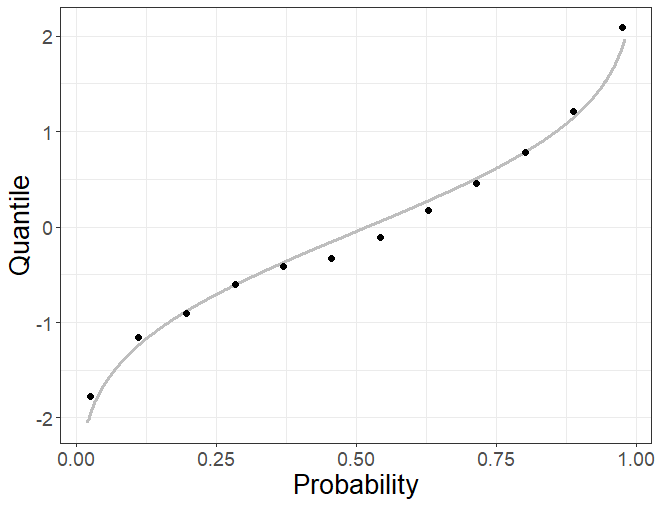
\includegraphics[scale=.5]{Images/fit_quantiles_example.png}
    \caption{Points representing 12 quantiles ($y$-axis) for given probability values ($x$-axis) estimated from a random sample of size 100 from a standard normal distribution. The quantile function (QF) of normal distribution (grey) was fit by selecting the mean and standard deviation parameters which minimize the least squares distance between the quantiles and the QF.}
    \label{fig:quant_match_example}
\end{figure}

Hereafter we refer to estimating a continuous distribution by fitting quantiles as quantile matching (QM).
\cite{sgouropoulos2015matching} performed QM by minimizing the mean square difference between quantiles of a response variable and a linear combination of quantiles of covariates. Selecting distribution parameters which minimize the mean square error
% \jarad{is least squares different than minimizing the mean square difference?}
between quantiles and a QF is a common QM method \cite[]{dilger2022distributions,li2019combining, belgorodski2017quantilemse}, 
% \jarad{Describe, briefly, what these methods do rather than just listing them.}
kernel density estimation and spline interpolation are common nonparametric QM methods \cite[]{gerding2023evaluating,gyamerah2020probabilistic,he2016short}, and \cite{keelin2016metalog} introduced a semiparametric method based on defining a flexible QF to fit quantiles. An issue shared by these methods is that they do not adequately account for the uncertainty inherent from the estimation of quantiles.  \cite{nirwan2020bayesian} introduced a QM model based on the definition of sample quantiles as order statistics and formulated
% \jarad{using as?}
the model likelihood as the joint PDF of multiple order statistics. This model provides exact inference for quantile uncertainty, but relies on the CDF and PDF of the distribution, making it less practical for fitting quantile defined distributions which have a QF but for which the CDF and PDF either do not exist in closed form or are difficult to evaluate \cite[]{perepolkin2023tenets,joiner1971some,tukey1960practical}. 
 


In this manuscript we introduce a novel model, the quantile Gaussian process (QGP), used specifically for QM. The context for using the QGP is that the available data is a set of quantiles estimated for a given set of probabilities.
The QGP relies on established theory underlying the relationship between the QF of a continuous distribution and sample quantiles \cite[]{parzen2004quantile, gilchrist2000statistical,hyndman1996sample,walker1968note,cramer1951mathematical}. The QGP can provide accurate asymptotic inference of uncertainty of quantiles, and it works well for QM for quantile defined distributions. 
In section \ref{sec:quant_func} the QF of a continuous random variable and sample quantiles are each defined, and important properties and asymptotic theory are reviewed. In section \ref{sec:qgp_model} the QGP model for QM is introduced. Section \ref{sec:simulation_analyses} contains simulation studies illustrating the QGP's ability to make parameter inference and match the distribution from which the quantiles where estimated. Section \ref{sec:qm_analysis} contains an application of QM using the QGP model for quantile forecasts of the 2023-24 United States Centers for Disease Control (CDC) flu forecasting competition, also known as FluSight. Section \ref{sec:qm_conclusion} concludes this manuscript with a short summary and ideas for further development in QM modeling.




\section{Quantile function and sample quantiles} \label{sec:quant_func}


Along with the CDF and PDF, the QF is a defining function of a random variable. The QF, however, often receives less attention in standard statistical training than do the CDF and PDF \cite[]{parzen2004quantile}, and the CDF and PDF are more used often for modeling and inference.
% But the QF tends to be the little brother 
% \jarad{little brother?}
% of both the CDF and PDF in that the latter two functions are taught and used far more in statistical modeling and inference. 
% Nevertheless, the QF and several of its properties are central to the QGP model introduced in this paper. 
% \jarad{another throwaway sentence}
This section contains the definition of the QF, important properties, the definition of sample quantiles, and key central limit theorems (CLTs) of sample quantiles. 

\subsection{Quantile function definition and properties}

The QF is defined in definition \ref{def:qf}.


\begin{definition}
    \label{def:qf}
    For a cumulative distribution function $F: \vmathbb{R} \rightarrow [0,1]$, the quantile function $Q: [0,1] \rightarrow \vmathbb{R}$ is defined as 
    
    \begin{equation*}
    \label{eq:qf}
        Q(p) = F^{-1}(p) := \emph{inf}\{x \in \vmathbb{R} : F(x) \geq p\}, \quad p \in [0,1]
    \end{equation*}
    An alternative definition not in terms of the cumulative distribution function is a function $Q: [0,1] \rightarrow \vmathbb{R} \cup \{-\infty, \infty\}$, which is nondecreasing and left-continuous. 
\end{definition}
% \jarad{the latter does not sound like a definition to me, but instead lists two properties.}

For most statistical applications, it is useful to define the QF as the inverse of the CDF. However, it is sometimes the case that defining a distribution by its QF first is advantageous, for instance when a distribution is defined by a QF but has no closed form CDF or when simple QFs may be aggregated to define more complex distributions \cite[]{perepolkin2023tenets, gasthaus2019probabilistic, alvarez2023quantile}. This section continues with important properties of the QF and functions including the location-scale property, the quantile density function, the probability integral transform, and examples of quantile defined distributions.
%(should the last reference be included??).

\subsubsection{Location-scale property}
For a random variable with PDF $f_0(x)$ and QF $Q_0(p)$ for $p\in [0,1]$, a location-scale family takes the PDF form $(1/\sigma)f_0((x - \mu)/\sigma)$ where the location parameter $\mu \in (-\infty, \infty)$ and the scale parameter $\sigma \in (0, \infty)$ \cite[]{casella2002statistical}. The QF of the location-scale family then takes the form $\mu + \sigma Q_0(p)$ \cite[]{parzen2004quantile}. By the addition and multiplication rules from section 3.2 of \cite{gilchrist2000statistical}, 
%(should I include a table listing properties somehwere??), 
this is a valid QF. \cite{gilchrist2000statistical} outlines the standardization rule which states that if the random variable $Y$ with QF $Q_Y(p)$ has a standard distribution, that is the random variable $Y$ is centered (by a mean or median) at 0 and has a scale of 1, then a random variable with quantile function $Q_{T(Y)}(p) = \mu + \sigma Q_Y(p)$ is centered at $\mu$ and has scale $\sigma$.

The linear form for a QF is already inherent in some distributions families such as the normal and logistic distribution families, with respective QFs $\mu + \sigma \Phi^{-1} (p)$ and $\mu + \sigma \text{log}(p/(1 - p))$. For the normal distribution, $\Phi^{-1}(p)$ is the QF of a standard normal distribution and $\mu$ and $\sigma$ are the mean and standard deviation of the location-scale transformed normal distribution. For the logistic distribution $\text{log}(p/(1-p))$ is the QF of a logistic distribution with mean 0 and scale 1, and $\mu$ and $\sigma$ become the mean and scale parameters of the location-scale transformed logistic distribution. The linear form is convenient for quantile regression modeling and is key to the development of the metalog distribution family which was designed specifically for modeling quantiles \cite[]{keelin2016metalog}. 
% Two examples of quantile defined distributions  are give further in this section.

\subsubsection{Quantile density function}

Besides the CDF, PDF, and QF a  fourth infrequently mentioned defining function of a continuous random variable is the quantile density function (QDF). As the PDF is the derivative of the CDF, the QDF $q:[0,1] \rightarrow \vmathbb{R}$ is the derivative of the QF defined as
\[
    q(p) = \frac{dQ(p)}{dp}.
\]
If $Q(p)$ is the inverse of a CDF $F(x)$, a calculus result shows that the reciprocal QDF $[q(p)]^{-1} = f(Q(p))$, or the PDF evaluated at the QF at $p$ \cite[]{perepolkin2023tenets, gilchrist2000statistical}. The QDF is important for establishing the CLTs in section \ref{sec:samp_quants} and for the QGP models introduced in section \ref{sec:qgp_model}.

\subsubsection{Probability integral transform}
An important application of the QF is using it to sample from continuous probability distributions via the probability integral transform (PIT). The PIT states that for any continuous random variable $Y$ with CDF $F_Y(y)$, the transformed random variable $X = F_Y(Y)$ is uniformly distributed on $(0,1)$, or $X \sim \text{Unif}(0,1)$. Thus if one can sample from a standard uniform distribution, one may also sample from a continuous distribution provided the QF of that distribution can be evaluated or reasonably approximated \cite[]{wilkinson2018stochastic}. The PIT is useful for assessing model fit via generalized residuals \cite[]{yang2024double, cox1968general} and the calibrating of probabilistic forecasts \cite[]{gneiting2007probabilistic}. Herein the PIT is important for developing one version of the QGP model, and it is used as part of a distance measure for assessing QM.

\subsubsection{Examples of quantile defined distributions} \label{sec:quant_def_dist}

An example of a quantile defined distribution family that lacks a CDF in closed form is the generalized lambda distribution (GLD) family \cite[]{ramberg1974approximate, perepolkin2023tenets}. A special case of the GLD family is the Tukey lambda distribution (TLD) family, a one parameter distribution family introduced by \cite{tukey1960practical}, \cite[]{joiner1971some}. The QF for the TLD is in (\ref{eq:tuk_lam}) and the QDF in (\ref{eq:tuk_lam_qd}).   

\begin{equation}
    \label{eq:tuk_lam}
    Q_{\lambda}(p) = \begin{cases} 
      \frac{1}{\lambda} \left[p^{\lambda} - (1 - p)^{\lambda} \right], & \lambda \neq 0 \\
      \text{log} \left(\frac{p}{1 - p} \right), & \lambda = 0
   \end{cases}
\end{equation}

\begin{equation}
    \label{eq:tuk_lam_qd}
    q_{\lambda}(p) = p^{\lambda - 1} + (1-p)^{\lambda -1} 
\end{equation}

Another distribution family defined by its quantile function but without a closed form CDF is the metalog distribution (MLD) family, a generalization of the logistic distribution family \cite[]{keelin2016metalog}. One version of the MLD is defined in (\ref{eq:mldq}).

\begin{equation}
    \label{eq:mldq}
    Q_{\textbf{a}}(p) = a_1 + a_3(p - 0.5) + a_2\text{log}\left(\frac{p}{1-p} \right)
\end{equation}
These two distributions will be used in section \ref{sec:simulation_analyses} for comparing different quantile matching methods.


















\subsection{Sample quantiles} \label{sec:samp_quants}

Using samples of a random variable to estimate quantiles is prevalent in statistical modeling. Given a random sample from some distribution, the sample quantile function may be defined in terms of the order statistics. \cite{hyndman1996sample} review several definitions of sample quantiles used in statistical packages and state definition \ref{def:sqf} as a general definition of the functions reviewed. 

\begin{definition}
For $n$ independent observations $Y_1, ..., Y_n$ from a distribution with corresponding order statistics $Y_{(1)}, ..., Y_{(n)}$, the sample quantile function $\hat{Q}_n(p)$ may be defined as
    \label{def:sqf}
    \begin{equation}
        \label{eq:quant_df}
        \hat{Q}_n(p) = (1- \gamma)Y_{(j)} + \gamma Y_{(j + 1)}
    \end{equation}
    where 
    \[\frac{j - m}{n} \leq p < \frac{j - m + 1}{n}
    \]
    for some $m \in \vmathbb{R}$ and $0 \leq \gamma \leq 1$ where $\gamma$ is some function of $j = \lfloor pn + m \rfloor$,  $g = pn + m - j$, and $\lfloor \cdot \rfloor$ is the floor function.
\end{definition}

Sample quantiles are used to give a probability summary of a dataset. Sample quantiles of Markov chain Monte Carlo draws from a Bayesian posterior distribution are used to analyze posterior distributions, for example by using quantiles to form credible intervals. 
Well known asymptotic results of sample quantiles are presented below, and it may be noted that asymptotic results for quantile regression quantiles are similar \cite[]{kocherginsky2005practical, koenker1978regression}. 
% (maybe rethink this statement or the specific citations??).

\subsubsection{Sample quantile central limit theorem} 

The asymptotic distribution of a set of sample quantiles is given in (\ref{eq:qclt}) and is the basis for the QGP model for QM in section \ref{sec:qgp_model}. For independent draws $Y_1, ..., Y_n$ from a continuous random variable with CDF $F$, PDF $f$, and QF $Q$, and with a set of sample quantiles calculated by (\ref{eq:quant_df}), theorem \ref{thm:qclt} holds. Note that in (\ref{eq:qclt}), $N_K(\cdot, \cdot)$ refers to a multivariate normal distribution with $K$ dimensions, and in (\ref{eq:qclt_covariance}) the operator $a \wedge b$ is the minimum of the values $a$ and $b$.

\begin{theorem}{\emph{Sample quantile central limit theorem}}
\label{thm:qclt}

Given a vector of length $K$ of probabilities $\boldsymbol{p} = (p_1, ..., p_K)$ and the corresponding quantile vector $\hat{\boldsymbol{Q}}_n(\boldsymbol{p}) = (\hat{Q}_n(p_1), ..., \hat{Q}_n(p_K))$, if $F$ is absolutely continuous for all $y \in \mathcal{Y}$ and is strictly increasing, then

\begin{equation}
    \label{eq:qclt}
    \sqrt{n}(\hat{\boldsymbol{Q}}_n(\boldsymbol{p}) - \boldsymbol{Q}(\boldsymbol{p})) \overset{D}{\rightarrow} N_K(0, \boldsymbol{\mathcal{K}})
\end{equation}
where $\boldsymbol{\mathcal{K}}$ is a $K\times K$ with the $ij^{th}$ entry $\kappa_{ij}$ where

\begin{equation}
    \label{eq:qclt_covariance}
    \kappa_{ij} = \frac{p_i \wedge p_j - p_i p_j}{f(Q(p_i)) f(Q(p_j))}
\end{equation}
\end{theorem}

Theorem \ref{thm:qclt} has been known since the mid 20th century \cite[]{cramer1951mathematical}, and a thorough though not unique proof is found in \cite{walker1968note}. The entries in the covariance matrix in (\ref{eq:qclt_covariance}) may equivalently be written as
\begin{equation}
    \rho_{ij} = [p_i \wedge p_j - p_i p_j]q(p_i)q(p_j)
    \label{eq:qgp_simp_cov}
\end{equation}
where $q$ is the QDF. Another CLT in (\ref{eq:tqclt}) for a set of quantiles transformed by the underlying CDF $F(\hat{\boldsymbol{Q}}_n(\boldsymbol{p})) = (F(\hat{Q}_n(p_1)), ..., F(\hat{Q}_n(p_k)))$ is in (\ref{eq:qclt}) and can be derived from (\ref{eq:qclt}) by using the PIT and the Delta method \cite[]{parzen2004quantile}.

\begin{equation}
    \label{eq:tqclt}
    \sqrt{n}(F(\hat{\boldsymbol{Q}}_n(\boldsymbol{p})) - \boldsymbol{p}) \overset{D}{\rightarrow} N_K(0, \boldsymbol{\Gamma})
\end{equation}
Here the covariance matrix $\Gamma$ has entries $\Gamma_{ij} = p_i \wedge p_j - p_i p_j$, making the asymptotic distribution in (\ref{eq:tqclt}) a Brownian bridge \cite[]{chow2009brownian}. This second result makes QM using the QGP model possible where $Q(p)$ is difficult to solve as is shown in the following section.




\section{Quantile Gaussian process model} \label{sec:qgp_model}

We consider the situation where one is given a set of data including a vector of $K$ probabilities $\boldsymbol{p} = (p_1, ..., p_K)$ and a vector of estimated quantiles at the given probability levels $\hat{\boldsymbol{Q}}_n(\boldsymbol{p}) = (\hat{Q}_n(p_1), ..., \hat{Q}_n(p_K))$. 
The set of quantiles may provide useful information about a distribution, but the information is limited and one may desire a more complete distribution.
The QDP model for QM and estimating a continuous distribution based on the CLT in (\ref{eq:qclt}) is in (\ref{eq:qgp}).



\begin{equation}
    \label{eq:qgp}
\hat{\boldsymbol{Q}}_n(\boldsymbol{p}) \sim N_K(\boldsymbol{Q}_{\theta}(\boldsymbol{p}), n^{-1} \boldsymbol{\mathcal{K}}_{\theta})
\end{equation}
Here $\theta$ is an unknown parameter to be estimated from the data. The covariance matrix $\boldsymbol{\mathcal{K}}_{\theta}$ has entries from the covariance function $\kappa_{\theta}(\cdot, \cdot)$ where 
\[
\kappa_{\theta}(p, p') = \frac{p\wedge p' - p p'}{f_{\theta}(Q_{\theta}(p)) f_{\theta}(Q_{\theta}(p'))}, \quad p, p' \in (0,1)
\]
Here the operator $a\wedge b$ indicates the minimum value between $a$ and $b$.

The covariance function $\kappa_{\theta} (\cdot, \cdot)$ initially appears as if it will be difficult to evaluate and indeed can be, depending on the functional forms of $f_{\theta}$ and $Q_{\theta}$. But where these functions belong to a location-scale family, the covariance function can be greatly simplified. 
Noting that the covariance is a function of $f_{\theta}(Q_{\theta}(p)) = q_{\theta}(p)$, the QDF, if $\theta = (\mu, \sigma)$ where $\mu$ is a location parameter and $\sigma$ is a scale parameter, then $q_{\theta}(p) = \sigma q(p)$ where $q(p)$ is the QDF of a standard distribution having location 0 and shape 1. \cite{staudte2017shapes} calls this the location invariant and scale equivariant property. For location-scale distribution families, this greatly simplifies the form of $\kappa_{\theta}(\cdot,\cdot)$ so that it becomes
\[
    \kappa_{\theta}(p, p') = \sigma^{2}[p\wedge p' - p p'] q(p)q(p') 
\] 
Thus for estimating $\theta$ one only needs to estimate $\sigma^2$. A special case of the QGP for QM of a location-scale family is the normal QGP which we define and explore below.


\subsection{Normal QGP}

If the quantiles in a dataset $(\hat{\boldsymbol{Q}}_n(\boldsymbol{p}),\boldsymbol{p})$ are assumed to be calculated from a normal distribution $N(\mu, \sigma^2)$, and the desire is to estimate the parameters $\mu$ and $\sigma$ by modeling the quantiles according to the QGP in (\ref{eq:qgp}), then one may use the model (\ref{eq:norm_qgp}). 

\begin{equation}
    \label{eq:norm_qgp}
\hat{\boldsymbol{Q}}_n(\boldsymbol{p}) \sim N_K \left( \mu + \sigma \boldsymbol{\Phi}^{-1}(\boldsymbol{p}),\frac{\sigma^2}{n} \boldsymbol{\Psi} \right)
\end{equation}
Here $\boldsymbol{\Phi}^{-1}(\boldsymbol{p}) = (\Phi^{-1}(p_1), ..., \Phi^{-1}(p_K))$ is a known vector since $\boldsymbol{p}$ is given, and $\boldsymbol{\Psi}$ is a known $K\times K$ matrix with $ij^{th}$ entry

\[
    \Psi_{ij} = \frac{2 \pi (p\wedge p' - p p')}{\text{exp}\{-\frac{1}{2}[\Phi^{-1}(p)^2 + \Phi^{-1}(p')^2]\}}.
\]
Model (\ref{eq:norm_qgp}) can then be viewed as an atypical normal linear regression model. Two aspects that make this model atypical relative to the standard linear regression model are that the slope parameter $\sigma$ must be greater than 0 and that $\sigma$ is both a regression coefficient and part of the variance.
% making $\sigma$ unidentifiable.
Note also that the sample size $n$ is included as part of the variance. If $n$ is known, then it may be multiplied through $\Psi$ and forgotten. If unknown, it can then be accounted for as an unknown part of the variance. 

Take for instance the data $\boldsymbol{X} = \left(\textbf{1}, \Phi^{-1}(\boldsymbol{p})\right)$ and the parameter vector $\beta = (\mu, \sigma)$. Assuming the sample size $n$ is unknown and setting $\sigma^2/n = \gamma^2$, model (\ref{eq:norm_qgp}) then becomes
\[
    \hat{\boldsymbol{Q}}_n(\boldsymbol{p}) \sim N_K\left(X\beta, 
\gamma^2 \boldsymbol{\Psi}\right)
\]
In this model, one simplifying assumption may be to treat $\sigma$ and $\gamma^2$ separately and proceed to fit a standard linear regression model. All frequentist and Bayesian results of the linear regression model apply, including the existence of conditionally conjugate prior distributions. The positive constraint on $\sigma$ can also be dealt with without adding much complication (see \cite{gelman2013bayesian} pgs. 377-378). If for a certain problem it is important to make inference on the unknown $n$, or $\sigma$ and $\gamma^2$ cannot treated as separate, then one may estimate the two parameters by assigning appropriate prior distributions to $\sigma$ and $n$ and reverting back to (\ref{eq:norm_qgp}). In section \ref{sec:simulation_analyses}, we analyze a normal QGP in a simulation study where we assign independent prior distributions to $\sigma$ and $n$, and $\sigma$ is treated as both a regression coefficient and as part of the variance.



For any QGP model where the QF belongs to a location-scale family, the discussed relation to the normal linear regression model applies. The only difference in modeling becomes formulating the matrix $\Psi$ using the proper QDF, and the data $\boldsymbol{X}$ with the proper quantile function. Many situations will require a more complicated QF which doesn't allow for modeling the data as a linear regression. Below we consider for instance a finite mixture distribution. 

\subsection{Finite normal mixture QGP}

For a continuous random variable distributed according to a finite mixture distribution, the CDF takes the form of (\ref{eq:norm_mix}). Here there are $C$ component distributions where $c \in \{1, ..., C\}$, $F_{\theta_c}$ is a continuous CDF with parameter $\theta_c$, and $w_c > 0$ is a weight such that $\sum_{c = 1}^C w_c = 1$. 

\begin{equation}
    \label{eq:norm_mix}
    F_{\theta}(x) = \sum_{c = 1}^C w_c F_{\theta_c}(x)
\end{equation}

Often $F_{\theta}$ will not be easily invertible, thus $Q_{\theta}$ will be a complicated function which can be evaluated only via numerical optimization which is often computationally expensive and/or inaccurate. A simple solution is to model the PIT transformed quantiles from the data rather than modeling the quantiles directly. The QGP model (\ref{eq:qgp}) is then reformulated to be model (\ref{eq:pit_qgp}), where  $\Gamma_{ij} = p_i\wedge p_j - p_i p_j$ as in (\ref{eq:tqclt}).   

\begin{equation}
    \label{eq:pit_qgp}
F_{\theta}(\hat{\boldsymbol{Q}}_n(\boldsymbol{p})) \sim N_K(\boldsymbol{p}, n^{-1} \boldsymbol{\Gamma})
\end{equation}

By modeling the PIT quantiles, the only function which requires evaluating is the CDF $F_{\theta}$. Here both $\boldsymbol{p}$ and $\boldsymbol{\Gamma}$ are given, and solving for the transformation $F_{\theta}(\hat{\boldsymbol{Q}}_n(\boldsymbol{p}))$ is unnecessary for our purposes. A Bayesian fit of (\ref{eq:pit_qgp}) is straightforward, requiring only that $F_{\theta}(\hat{\boldsymbol{Q}}_n(\boldsymbol{p}))$ be evaluated as part of the acceptance ratio of a Markov chain Monte Carlo (MCMC) iteration. 

In section \ref{sec:simulation_analyses}, we analyze PIT transformed QGP model (\ref{eq:pit_qgp}) where $F_{\theta}$ is set as a normal mixture distribution with $C = 4$ component normal distributions. Fitting this model proved faster and produced better results than trying to fit the QGP model (\ref{eq:qgp}) and evaluating $Q_{\theta}$ the QF of a normal mixture. In fact we found that in cases where $F_{\theta}$ was a simpler function, such as a normal or exponential distribution, fitting model (\ref{eq:pit_qgp}) was at least as fast and the results were at least as good as fitting (\ref{eq:qgp}). Thus when possible, we elected to fit (\ref{eq:pit_qgp}).  



 




\subsection{Competing quantile matching methods}

A number of methods already exist for QM. Here we briefly review four of those methods, and in section \ref{sec:simulation_analyses} we compare performance between these and the QGP. The four methods include spline interpolation (SPL), kernel density estimation (KDE), an order statistics based model (ORD), and an independent quantile model (IND). The first two of these methods are non-parametric methods and neither of which include modeling the uncertainty of the quantiles.

The SPL method was used by \cite{gerding2023evaluating} and \cite{shandross2024hubensembles} in order to estimate a CDF function given quantile forecasts from disease outbreak forecast hubs. SPL is an interpolation where monotonic cubic splines are fit to pass through each given quantile and predict a function for all values between given quantiles and beyond the extreme values. An \texttt{R} package used for fitting SPL and which we use in section \ref{sec:simulation_analyses} is \texttt{distfromq} \cite[]{ray2024quantmatch}.

The KDE method treats given quantiles as if they constitute a random sample from a distribution and applies kernel smoothing to estimate a density function. KDE requires selecting a kernel function, often a Gaussian kernel is chosen, and applying that function to each draw in a sample. \cite{gyamerah2020probabilistic} applied KDE smoothing with an Epanechnikov kernel to quantiles estimated via three different machine learning methods used for predicting crop yield. They then combined the estimated densities into an ensemble prediction. \cite{he2016short} also use KDE to estimate density forecasts from quantiles to produce energy forecasts. We use the \texttt{evmix} package for performing QM using KDE \cite[]{yang2018kde}.

One of the more common methods for QM is to select a CDF or QF function and then select model parameters which give a least squares fit to the estimated quantiles as done by \cite{li2019combining}. 
% and \cite{wadsworth2023mixture}. 
The \texttt{R} package \texttt{rriskDistributions} performs this least squares fit for some standard distributions \cite[]{belgorodski2017quantilemse}. Independent random error may be included to the best fit QF allowing for estimation of the variability of the quantiles \cite[]{nirwan2020bayesian}. In section \ref{sec:simulation_analyses}, we analyze model (\ref{eq:ind_quantile}) as a proxy for the IND model to compare with other methods. 
\begin{equation}
    \label{eq:ind_quantile}
    F_{\theta}(\hat{Q}(p_k)) \overset{ind}{\sim} N(p_k, \sigma_{\rho}^2)
\end{equation}
Here $\hat{Q}_k$ is the estimated sample quantile at probability $p_k$. The major difference between model (\ref{eq:ind_quantile}) and model (\ref{eq:pit_qgp}) is that the error for each quantile in a set of quantiles is considered independent, and the effects of sample size and correlation suggested by the CLT in (\ref{eq:tqclt}) are ignored. Note that the parameter $\sigma_{\rho}$ is not a part of $\theta$, the parameter of the ``true" distribution estimated by QM but instead is meant to capture independent error among the sample quantiles.





The final method we include is the ORD model introduced by \cite{nirwan2020bayesian}. This model relies on the definition of sample quantiles being order statistics. In the ORD model, the joint distribution of a set of order statistics is the model likelihood. The likelihood of a set of order statistics from a continuous distribution is a function of both the CDF and PDF of a continuous distribution. ORD is the method most similar to QGP and it provides exact inference of quantile uncertainty whereas the QGP provides asymptotic inference of uncertainty. 

For assessing QM, there are two aspects we analyze. The first is a model's ability to estimate parameters and the second is how far away a fit QM distribution is from a true distribution. Of the methods previously listed, parameter inference is only possible for the QGP, IND, and ORD models. These are also the only methods which provide uncertainty quantification for quantile values. To analyze how far an estimated distribution is from a true distribution, a distance measure must be utilized. We outline three of these distances below.

\subsection{Distance measures}

A number of metrics for measuring the distance between two continuous univariate distributions exist. Those we consider in this paper are the Wasserstein distance (WD) and a slight modification of it, the total variation (TV) or the statistical difference, and the Kullback-Leibler divergence (KLD). A brief overview of these and other metrics, some of their statistical uses and properties, and relationships between metrics is found in \cite{gibbs2002choosing}. These metrics were used in section \ref{sec:simulation_analyses} to assess the how well different QM methods approximate a true distribution.


% \subsubsection*{Wasserstein distance}
The WD is used to measure the distance between two univariate random variables by their CDFs or QFs and has many applications in mathematics, optimization, and statistics, see \cite{panaretos2019statistical} for a review of the WD and its use in statistics. The $p$-WD is defined for two continuous random variables $X$ and $Y$ with respective CDFs $F_X$ and $F_Y$. In terms of the two CDFs the $p$-WD is defined in (\ref{eq:wass_dist_cdf}), and the $p$-WD in terms of the corresponding QFs is defined in (\ref{eq:wass_dist_quant}). 

\begin{equation}
    \label{eq:wass_dist_cdf}
    WD_p (F_X, F_Y) = \left( \int_{\vmathbb{R}} |F_X(t) - F_Y(t)|^p dt\right)^{1/p}
\end{equation}

\begin{equation}
    \label{eq:wass_dist_quant}
    WD_p (F, G) = \left( \int_0^1 |F^{-1}_X(t) - G^{-1}_Y(t)|^p dt \right)^{1/p}
\end{equation}

We define a modified version of the WD, the uniform 1-WD (UWD1) in (\ref{eq:pit_wass_dist}). Here we take $F_X$ to be the CDF of a continuous random variable $X$. For a different continuous random variable $\xi$ with CDF $F_{\xi}$, $F_X(\xi)$ is a random variable with support on $[0,1]$. We let $F_{X,\xi}$ be the CDF of the random variable $F_X(\xi)$. Then the measure in (\ref{eq:pit_wass_dist}) is a measure of how close $F_X(\xi)$ is the the CDF of a standard uniform distribution, noting that by the PIT, if $\xi \overset{D}{=} X$, $F_X(\xi)$ is the random variable of a standard uniform distribution. Multiplying the integral in (\ref{eq:pit_wass_dist}) by two ensures the measure takes values between 0 and 1 \cite[]{645854} where a value near 0 means $\xi$ and $X$ are "near" each other.

\begin{equation}
    \label{eq:pit_wass_dist}
    UWD_1(F, \mathcal{L}) = 2\int_0^1 |F_{X,\xi} (x) - x|dx
\end{equation}


% \subsubsection*{Total variation}

The TV, defined in (\ref{eq:tot_var}), is a distance between distributions measured in terms of the PDFs $f$ and $g$. The TV takes values between 0 and 1, and it is closely related to the distance used in \cite{sgouropoulos2015matching} to measure the goodness of QM.  

\begin{equation}
    \label{eq:tot_var}
    TV(f,g) = \frac{1}{2} \int_{-\infty}^{\infty}|f(x) - g(x) | dx
\end{equation}

% \subsubsection*{Kullback-Leibler divergence}

The final metric between distributions we consider is the KLD defined in (\ref{eq:kld}). The KLD is not a true metric but has many useful properties and applications. It may be interpreted as the expected divergence if one is using $f$ to approximate $g$. 


\begin{equation}
    \label{eq:kld}
    KLD(g || f) = \int_{\mathcal{X}} g(x) \text{log} \left( \frac{g(x)}{f(x)} \right) dx
\end{equation}



\section{Quantile matching methods comparison on simulated data} \label{sec:simulation_analyses}

In this section we present several simulation studies assessing the QM of the QGP model and compare results with those of the SPL, KDE, IND, and ORD matching methods. The QGP, IND, and ORD models were each fit via Hamiltonian Monte Carlo (HMC) sampling using the \texttt{Stan} software and the \texttt{cmdstanr} package developed and maintained by the \cite{stan2024manual} \cite[]{gabry2022stan}. Simulation studies are done to assess parameter estimation and inference as well as QM estimation of a distribution.



\subsection{Parameter estimation and quantile matching for known distribution \\families} 

Where the distribution family is known, one goal of QM may be to estimate and make inference on model parameters. In the first two studies, we analyzed parameter estimation and inference for normal and exponential family distributions with known parameters. We analyzed the QGP model from (\ref{eq:pit_qgp}), the IND model, and the ORD model. We note that model (\ref{eq:pit_qgp}) allows one to do inference for both the model parameter $\theta$ and for an unknown sample size $n$. The ORD model also allows for estimation of an unknown $n$. For the QGP and ORD models, we include modeling cases where $n$ is known and where $n$ is unknown and estimated. We denote the models where $n$ is known as QGP-n and ORD-n. We also compared the distance between the true model and the predictive distributions estimated via QGP, IND, ORD, SPL, and KDE. We also include a comparison of the QGP and ORD models where the true distribution is a quantile defined distribution.

\subsubsection{Normal parameter estimation}
In this simulation study we fit the ORD and IND models to quantiles estimated from independent samples from a normal distribution and compare parameter estimation with fits from the QGP model. Quantiles were simulated by first drawing a sample of size $n$ from a known distribution then estimating $K$ quantiles given probabilities $\{p_1, ..., p_K\}$. The ORD, IND, and QGP models were then fit to the quantiles where $F$ was set to be the CDF of a normal distribution. For each combination of $n \in \{50, 150, 500, 1{,}000, 5{,}000\}$ and $K \in \{3,7,15,50\}$, there were 500 simulation replicates. The data were simulated from a normal distribution with mean $\mu = 4$ and standard deviation $\sigma = 3.5$.
For each of QGP, ORD, and IND models, we assigned the same prior distributions to $\mu$ and $\sigma$. When $n$ is unknown, we also assigned it a prior distribution. The prior distributions were

\begin{align*}
    \mu &\sim N(5,7^2) \\
    \sigma &\sim N(0, 6^2) \vmathbb{1}\{\sigma > 0\}\\
    n &\sim N(0,3000^2)\vmathbb{1}\{n > 0\}.
\end{align*}
For the IND model the prior on the independent parameter $\sigma_{\rho}\vmathbb{1}\{n > 0\}$ from model (\ref{eq:ind_quantile}) is $1/\sigma_{\rho} \sim N(0, 3000^2)$, which is similar to the prior on $n$ for the QGP and ORD models. For each fit, the HMC chain was run for 60,000 draws with the first 10,000 discarded as a burn-in.

Figure \ref{fig:normal_densities} shows examples of marginal posterior densities for $\mu$, $\sigma$, and unknown $n$ where the true $n \in \{50,\,150,\,500,\,1,000\}$ and $K \in \{7,\,15,\,23\}$. 
The parameter uncertainty of the QGP and ORD models are unsurprisingly similar in most cases, and where they differ it is hard to say that one is estimating the true parameter better than the other. The IND model on the other hand has tighter densities, and often the bulk of the posterior is far from the true parameter.
\begin{figure}[hbt!]
% \begin{subfigure}{.475\linewidth}
  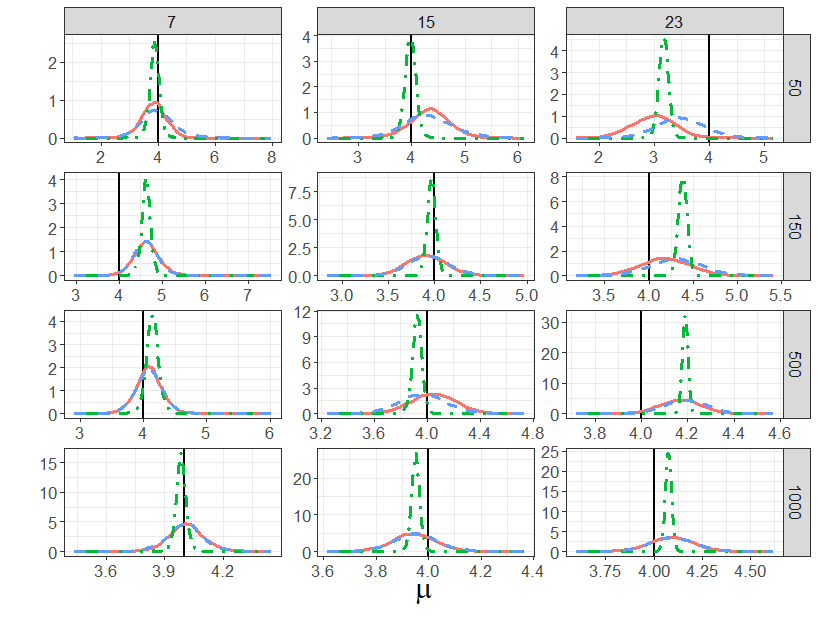
\includegraphics[width=.4\linewidth]{Images/normal_mean_fit.png}
  % \caption{}
  % \label{MLEDdet}
% \end{subfigure}\hfill % <-- "\hfill"
% \begin{subfigure}{.52\linewidth}
  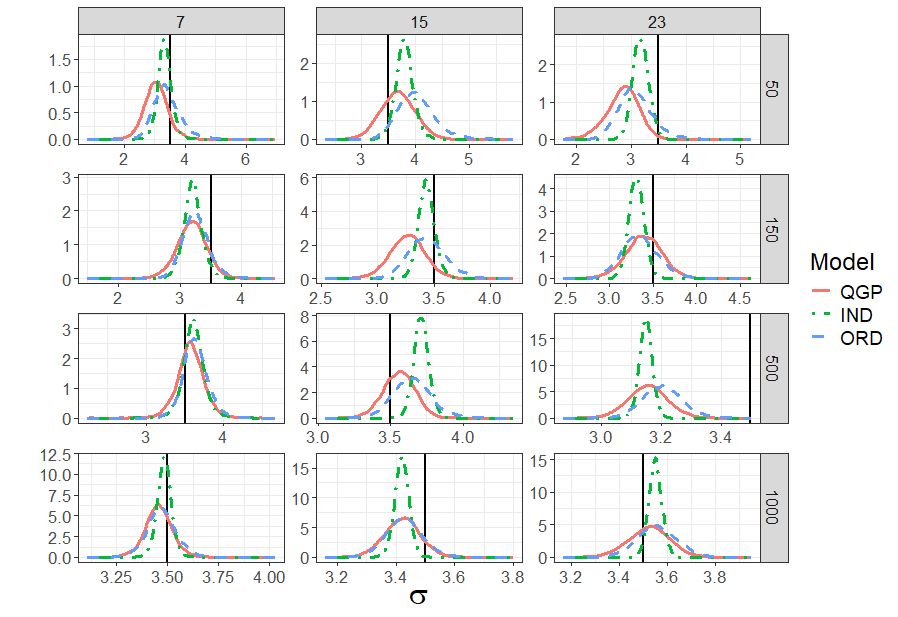
\includegraphics[width=.4\linewidth]{Images/normal_sd_fit.png}
  % \caption{}
  % \label{energydetPSK}
% \end{subfigure}

\medskip % create some *vertical* separation between the graphs
%\begin{subfigure}{.53\linewidth}
  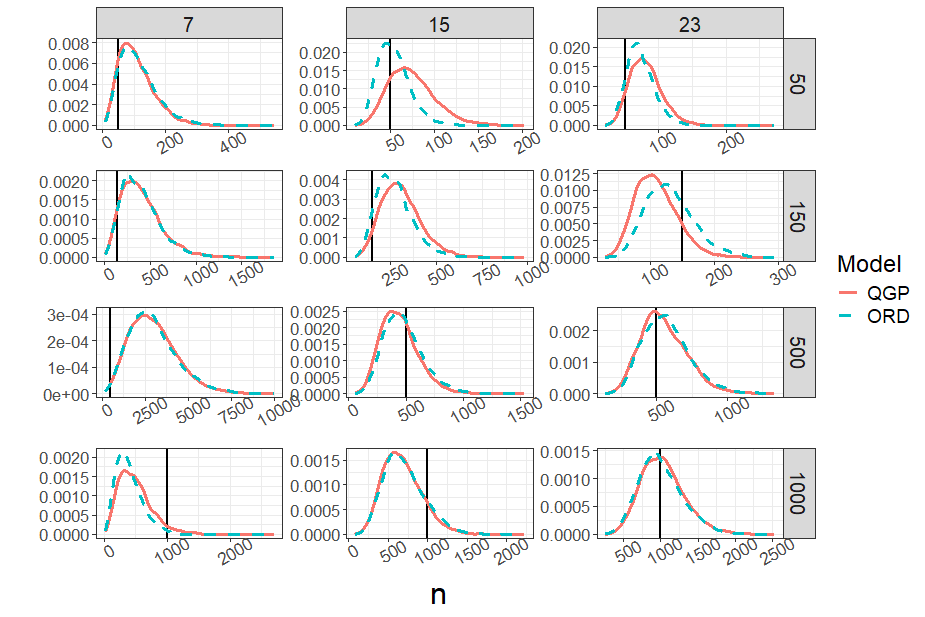
\includegraphics[width=.4\linewidth]{Images/normal_n_fit.png}
  % \caption{}
  % \label{velcomp}
%\end{subfigure}\hfill % <-- "\hfill"
\tiny
\caption{Density plots of posterior distribution samples for normal parameters by QM for QGP, ORD, and IND models. QM was done on estimated quantiles from a normal distribution with mean 4 and standard deviation 3.5. The posterior densities are for $\mu$ (top left), $\sigma$ (top right), and sample size $n$ (bottom). Plots are faceted by the sample size $n \in \{50, 150, 500, 1{,}000\}$ ($y$-axis) and number of quantiles $K \in \{7, 15, 23\}$ ($x$-axis). Vertical lines (black) show the value of the true parameter.}
\label{fig:normal_densities}
\end{figure}


The left side of figure \ref{fig:normal_cov_dists} shows the 90\% coverage of the posterior distribution credible intervals as $n$ increases for $\mu$, $\sigma$ and $n$ for five models. QGP-n and ORD-n models where $n$ is known are included along with QGP, ORD, and IND. 90\% credible intervals of the parameters were calculated by computing the $0.05^{th}$ and $0.95^{th}$ quantiles from the posterior distribution samples. The coverage percentage is calculated as the percentage of the 500 replicates which the true parameter value was within the 90\% credible interval.
As expected, the nominal coverage for the QGP and ORD models is better than that of the IND model, and for the two models where $n$ is known the coverage is better than where it is unknown, particularly for lower values of $n$ and $K$. The coverage for the ORD models appears to be slightly better than for the QGP models though not by much and not for every combination of $n$ and $K$. This is likely because the ORD model provides exact inference whereas the QGP model provides asymptotic inference.



\begin{figure}[hbt!]
%\begin{subfigure}{.465\linewidth}
  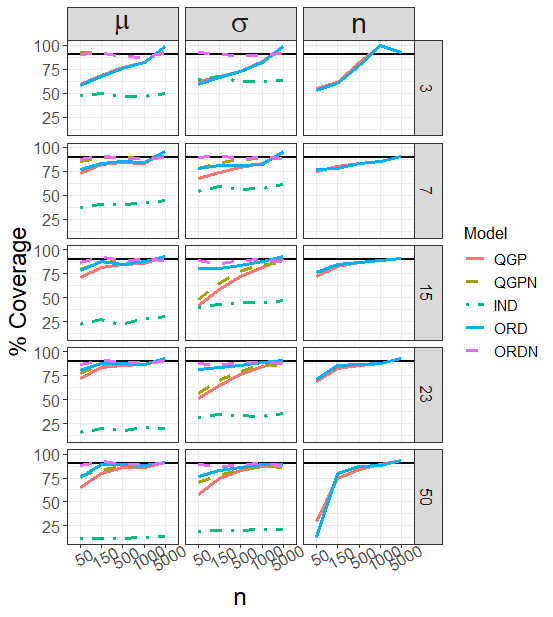
\includegraphics[width=.4\linewidth]{Images/normal_coverage.png}
  % \caption{}
  % \label{MLEDdet}
%\end{subfigure}\hfill % <-- "\hfill"
%\begin{subfigure}{.524\linewidth}
  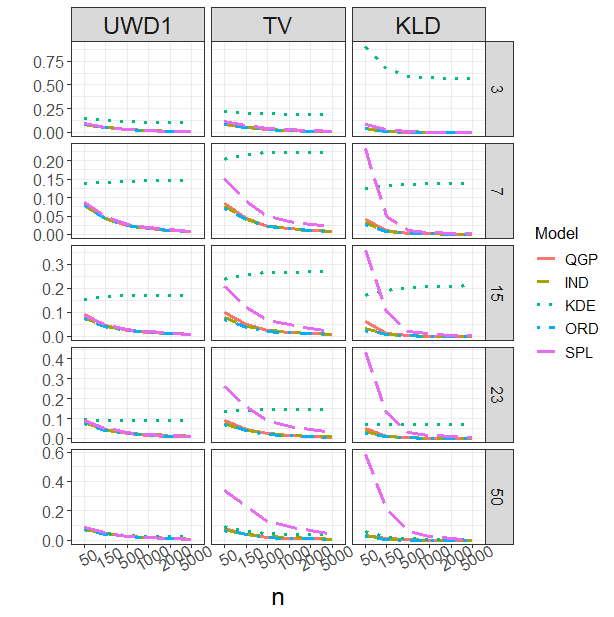
\includegraphics[width=.4\linewidth]{Images/normal_dists.png}
  % \caption{}
  % \label{energydetPSK}
%\end{subfigure}
\caption{Posterior coverage (left) calculated as the percentage of times the true parameter fell within the modeled 90\% credible interval over the 500 replications. Coverage is faceted by the normal parameters $\mu$, $\sigma$, and $n$ with $K \in \{3, 7, 15, 23, 50\}$, and by increasing sample size ($x$-axis). The five models QGP, ORD, QGP-n, ORD-n, and IND are colored as shown the legend. The horizontal line (black) is at the nominal 90\% level. Only QGP and ORD appear for the parameter $n$ as they are the only two which estimate an unknown $n$.
Distance between the true distribution and the estimated QM predictive distribution (right) averaged over the 500 replications. Distances include the UWD1, TV, and KLD for $K \in \{3, 7, 15, 23, 50\}$, and by increasing sample size ($x$-axis).}
\label{fig:normal_cov_dists}
\end{figure}



To analyze how well QM methods produced predictive distributions which approximate the true distribution $N(4, 3.5^2)$, we measured the distance between the estimated predictive distributions of QGP, ORD, and IND fits to the true distribution. 
We also measured the distances of the SPL and KDE QM fits to the true distribution. The distances were measured via the UWD1, TV, and KLD metrics. 
The UWD1 for each of QGP, ORD, QGP-n, ORD-n, and IND were calculated as follows. For $\{\theta_m\}^M$ being $M$ draws from the posterior distribution of $\theta$ where $\theta_m = (\mu_m, \sigma_m)$, the QM posterior predictive distribution was simulated by repeatedly sampling a $\theta_m^*$, then sampling $X_m$ from a distribution with CDF $F_{\theta_m^*}$. Repeating this for $M = 50,000$ times gives a QM posterior predictive sample. For the CDF $F_{\theta}$ where $\theta$ is the true parameter, $\xi_m = F_{\theta}(X_m)$ was calculated and the empirical CDF $\hat{F}_{\xi}$ was calculated from the sample $\{\xi_m\}^M$. $F_{\xi}$ in (\ref{eq:pit_wass_dist}) was then replaced by $\hat{F}_{\xi}$ to calculate UWD1. For SPL and KDE $F_{\xi}(x)$ was replaced by the respective estimated CDFs. The \texttt{integrate} function in \texttt{R} was used for calculating the UWD1 in (\ref{eq:pit_wass_dist}).

To estimate TV and KLD, rather than sampling from the posterior distribution, the marginal means for the parameters were calculated from the posterior distribution samples. These marginal means  are $\Bar{\theta}_M = (\Bar{\mu}_M, \Bar{\sigma}_M)$ where $\Bar{\mu}_M$ and $\Bar{\sigma}_M$. To calculate TV, $f$ in (\ref{eq:tot_var}) is replaced by $f_{\Bar{\theta}_M}$ and $g$ is replaced by $f_{\theta}$. The TV calculation was done using the \texttt{integrate} function in \texttt{R}. The KLD was estimated also using $f_{\Bar{\theta}_M}$ and $f_{\theta}$, but was done via Monte Carlo sampling. That is (\ref{eq:kld}) was estimated by

\[
    \widehat{KLD}(f_{\theta} || f_{\Bar{\theta}_M}) = \frac{1}{S}\sum_{s = 1}^S \text{log} \left(\frac{f_{\theta}(Y_s)}{f_{\Bar{\theta}_M}(Y_s)}\right)
\]
where $Y_s \overset{iid}{\sim} F_{\theta}$. For both SPL and KDE, $f_{\Bar{\theta}_M}$ is the estimated PDF.


The right side of figure \ref{fig:normal_cov_dists} shows the UWD1, TV, and KLD metrics averaged over the 500 simulation replicates as $n$ increases for the five QM methods. The QGP, ORD, and IND are nearly indistinguishable and outperform the SPL and KDE in almost every case, though KDE tends to improve as $K$ increases, performing similar to the parametric methods for $K = 50$. For UWD1, the SPL performs similarly to the parametric QM methods, but for the TV and KLD, the SPL performs much worse, especially for smaller sample sizes. 

This study shows the ability of the QGP QM model to estimate and perform inference on model parameters where the true distribution family is known. It also shows the QGP's ability to produce a posterior predictive distribution which closely matches a true distribution, according to several metrics, relative to other QM methods. Between parameter inference and predicting the true distribution, QGP is superior to all methods we compared it with except for the ORD model which has similar results to the QGP. A similar simulation study where the data is simulated from an exponential family distribution is in appendix 
% \ref{app:extra_sim}. 
The results of that study are similar to those of the normal distribution family study.




When fitting the Bayesian models both in the normal and in the exponential setting, the IND model tended to fit the fastest, followed by the ORD models, and finally the QGP models. The time to fit however was very fast, usually no more than seven seconds except for the case where $K = 50$ quantiles, in which case the QGP model where $n$ was unknown often took around 20 seconds to fit. However, with $K= 50$ the QGP-n model continued to fit very rapidly, fitting in under seven seconds.

The analysis above show the usefulness in using the QGP model both in parameter estimation and in QM when given sample quantiles. In the normal case, the QGP showed improved parameter inference over the IND model and allows for making inference on the sample size $n$. Compared to the SPL and KDE QM methods, the QGP fits tend to be closer in distance to the true distribution. The QGP model, however, performs about the same as the ORD model in terms of inference and QM. The section below outlines a situation where the QGP model may be a better option for QM than the ORD model. 


\subsubsection{Quantile defined distributions}
The normal and exponential families both have CDF and PDF functions which are either available in closed form or are easy to evaluate with software which is widely accessible. The next study we performed was done to compare the QGP and ORD models where the distribution family was a quantile defined distribution which lacks a CDF that is easy to evaluate. The purpose of this study was to show an example where one may prefer to perform QM using the QGP rather than the ORD.


The GLD is reviewed in section \ref{sec:quant_def_dist}, and a simulation carried out similarly to the previous studies was performed with GLD as the true distribution. However, QM was only done by the QGP and ORD models. Because of the relative difficulty of evaluating the CDF of the GLD and the ease of evaluating the QF, the CDF transformed QGP model in (\ref{eq:qgp}) instead of (\ref{eq:pit_qgp}) was used. For the ORD model, evaluating the CDF was required for modeling. Evaluating the CDF of the GLD requires using an algebraic solver, and it took longer to code the ORD model in \texttt{Stan} due to there not being readily available software which we were aware of. Once working, however, both QGP and ORD models fit the estimated quantiles well, however, the ORD usually required more time to fit than the QGP. Figure \ref{fig:tuk_time} shows boxplots for the 500 replicates for different values of $K$ quantiles. In all cases except for $K=50$ the QGP tends to fit much faster than ORD. Note that the $y$-axis is on the logarithmic scale. Even at $K=50$ some outliers for the ORD model required thousands of seconds to fit whereas the longest required time for fitting a QGP model was a few hundred seconds.


\begin{figure}[hbt!]
    \centering
    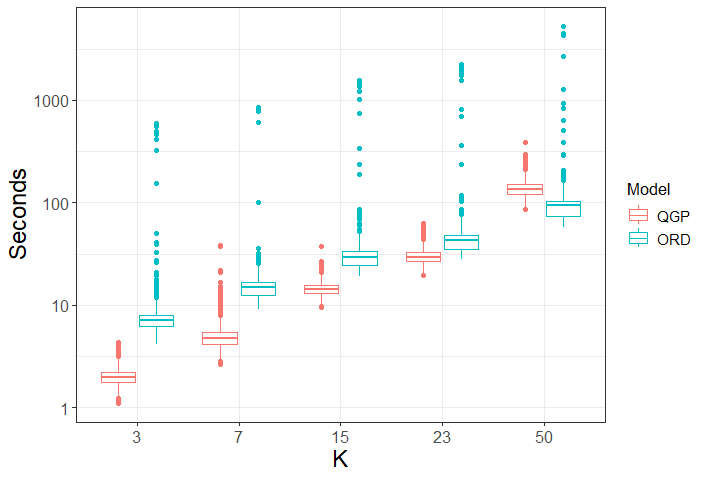
\includegraphics[scale=.6]{Images/tukey_time_log10.png}
    \caption{Boxplots of time to fit a model in seconds ($y$-axis) for the 500 replicates in the simulation study for QM of the generalized lambda distribution (GLD) for $K \in \{3, 7, 15, 23, 50\}$ ($x$-axis). Boxplots are separated by QM methods QGP (red) and ORD (blue). The $y$-axis is on the $\text{log}_{10}$ scale.}
    \label{fig:tuk_time}
\end{figure}

 The MLD was also reviewed in section \ref{sec:quant_def_dist}. We were able to fit a QGP model for the MLD which appeared to fit sample quantiles well, but we were unable to fit a working ORD model. The algebraic solver struggled to evaluate the CDF, and posterior sampling in \texttt{Stan} was extremely slow. When fitting finally finished, the result was a very poor fit. Perhaps with more time and effort we could have made a working model, but the QGP worked well enough that we did not feel it was worth the effort.





\subsection{Matching unknown distributions} \label{sec:uk_matching}

The simulation studies in this section are for the situation where the true distribution family is unknown, unimportant, or too complex to be practically evaluated but where one still wishes to recover or approximate the distribution. We selected three distributions each with a different shape to analyze how well the distributions can be approximated by QM using the QGP and the competing methods. 

With the true distribution family being unknown, we made the modeling decision to set $F$ in the QGP model of (\ref{eq:pit_qgp}) to be a mixture of normals distribution taking the form of (\ref{eq:norm_mix}). The number of component distributions was chosen to be $C = 4$ to provide enough flexibility to approximate the different shapes of quantile functions. This decision was based on the common claim that any continuous distribution may be approximated by a finite mixture of normal distributions \cite[]{peel2000finite,nguyen2019approximations,nguyen2020approximation}. This claim may be optimistic, but we found that a four component normal mixture distribution can approximate the non-normally shaped distributions reasonably well. However, any function which meets the technical definition of a CDF would be appropriate to use for $F$, see \cite{gasthaus2019probabilistic} for an example.



The three distributions from which data were simulated and sample quantiles estimated and to which QM methods were fit were the extreme value (EV) distribution with location 0 and scale 1 $EV(0,1)$, Laplace (LA) with location 0 and scale 1 $La(0,1)$, and a two component normal mixture (MIX) $w N(-1, 0.9) + (1-w)N(1.2, 0.6)$ where $w = 0.35$. From the three distributions, 500 replicates of $K$ quantiles were simulated for each of 
$K \in \{9, 13, 23, 50\}$ and sample size $n \in \{50, 150, 500, 1{,}000, 2{,}000, 5{,}000\}$. QM for each replicate of simulated quantiles was done using QGP, ORD, IND, SPL, and KDE. For the QGP, ORD, and IND models, $\theta = \{\theta_1, \theta_2, \theta_3, \theta_4\}$ where $\theta_c = (\mu_c, \sigma_c)$ for $c \in \{1,2,3,4\}$. The prior distributions assigned were as below where $\nu = n$ for the QGP and ORD models and $\nu = 1/\sigma_{\rho}$ for the IND model. 
% (cite an example of using dirichlet prior ??). 

    \begin{align*}
        \mu_c &\overset{ind}{\sim} N(5, 7^2) \\
        \sigma_c &\overset{ind}{\sim} N(0, 6^2)\vmathbb{1}\{\sigma_c > 0\} \\ 
        w &\sim Dir(\boldsymbol{\alpha}), \quad \alpha_c = 1 \\
        \nu &\sim N(0, 3000^2)\vmathbb{1}\{\nu > 0\}
    \end{align*}
 %the problem with $\nu$ is that for the QGP and ORD the prior is on the variance whereas for IND it is on the sd.
Often when implementing posterior sampling for a mixture distribution model, one deals with an issue called the label-switching problem. This is where for a mixture distribution parameter $\theta = \{\theta_1,...,\theta_C\}$, the model likelihood is the same for different permutations of $\theta$. This lack of identifiability for elements of $\theta$ makes parameter inference useless, but the predictive distribution may still be close to the true distribution \cite[]{stephens2000dealing}.
Because of this, the HMC posterior sampling chain was run longer than in the studies in the previous section. The chain was run for 80,000 steps where the first 20,000 draws were discarded as a burn-in. For this study, we were concerned only with QM and not with parameter inference, so the fact that the parameters are unidentifiable was not considered critical. However, when assessing the TV and KLD between the QM and true distributions, variational Bayes (VB) in \texttt{Stan} was used instead of HMC for fitting the models \cite[]{kucukelbir2015automatic}. This decision was made because of the lack of parameter identifiability and because the marginal parameter means are used to estimate the PDF. While MCMC methods perform better on parameter inference, VB methods have been shown to have predictive performance comparable to MCMC \cite[]{blei2017variational}.


Figures \ref{fig:evd_fits}, \ref{fig:lp_fits},  and \ref{fig:gmix_fits} each show examples of fits of $K=23$ quantiles simulated from the EV, LA, and MIX distributions respectively for different sample sizes $n$. Included QM methods are KDE, SPL, IND, and QGP. ORD was excluded to make visualization easier, but the fits are very similar to the QGP fits. The KDE and SPL fits provide no uncertainty estimation of the quantiles, and return only a continuous function. The SPL fits show a lot of wiggle with the wiggle decreasing as $n$ increases, whereas the KDE fits do not show as much wiggle, but the KDE fits the distribution tails poorly even as $n$ increases. The IND and QGP models provide uncertainty in the fits, but the QGP is much more conservative with wider intervals which provide superior coverage of the quantiles and the PDFs. 







\begin{figure}[hbt!]
\centering
%\begin{subfigure}{.5\textwidth}
  \centering
  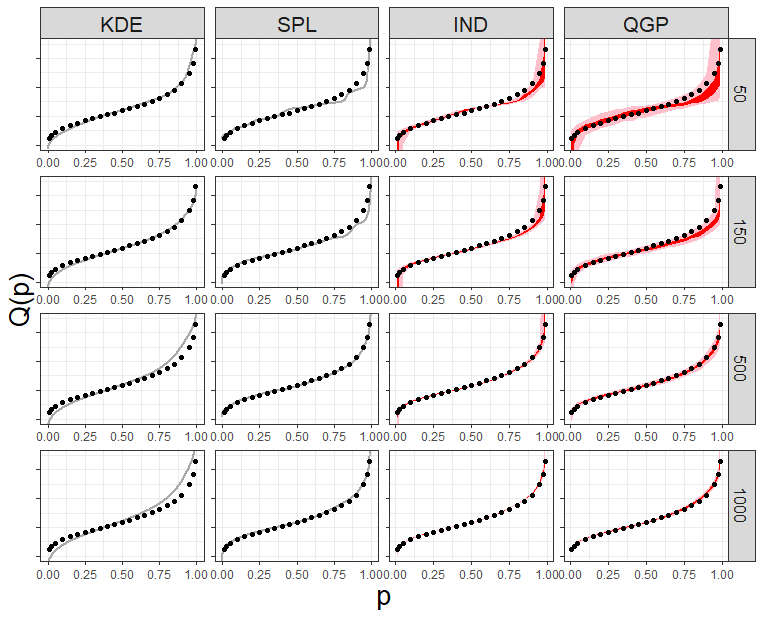
\includegraphics[width=.49\linewidth]{Images/quants_evd.png}
  % \caption{A subfigure}
  % \label{fig:sub1}
%\end{subfigure}%
%\begin{subfigure}{.5\textwidth}
  \centering
  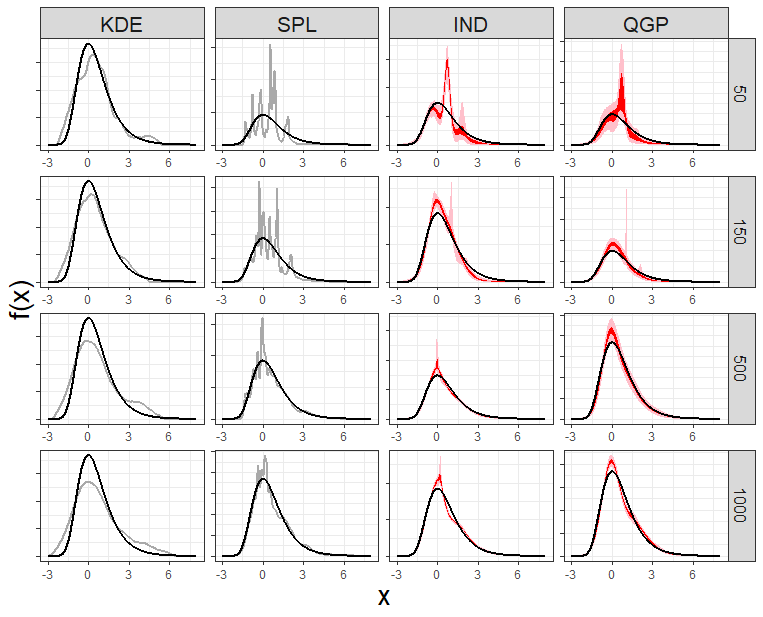
\includegraphics[width=.49\linewidth]{Images/dens_evd.png}
  % \caption{A subfigure}
  % \label{fig:sub2}
%\end{subfigure}
\caption{QM fits of $K=23$ quantiles by KDE, SPL, IND, and QGP for $n \in \{50, 150, 500, 1{,}000\}$. The quantiles were sampled from the extreme value distribution $Ev(0,1)$. The quantile fits (left) show the true quantiles (black) with either the QM fit line (grey) or the credible intervals of 50\% (red) and 95\% (pink). 
The estimated PDF plots (right) show the true PDF (black) with either a the QM estimated PDF (grey) or the credible intervals of 50\% (red) and 95\% (pink).}
\label{fig:evd_fits}
\end{figure}

\begin{figure}[hbt!]
\centering
%\begin{subfigure}{.5\textwidth}
  \centering
  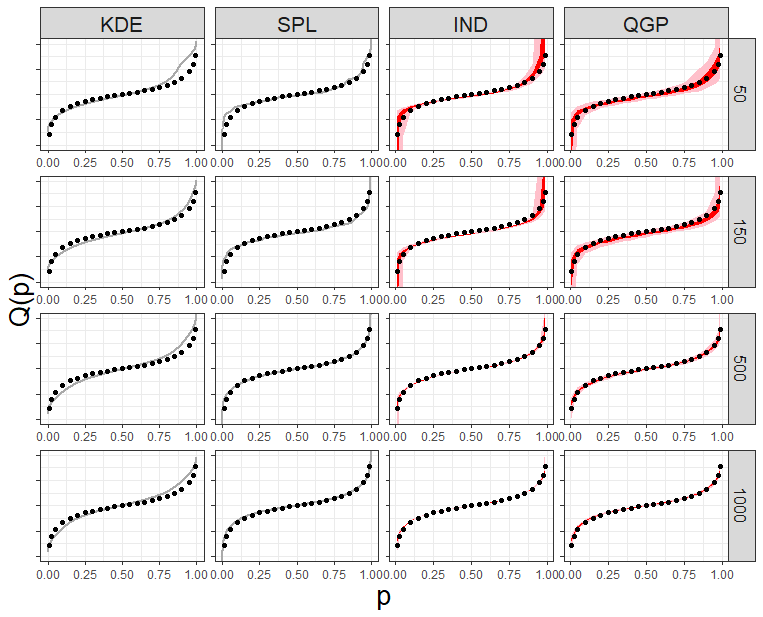
\includegraphics[width=.49\linewidth]{Images/quants_lp.png}
  % \caption{A subfigure}
  % \label{fig:sub1}
%\end{subfigure}%
%\begin{subfigure}{.5\textwidth}
  \centering
  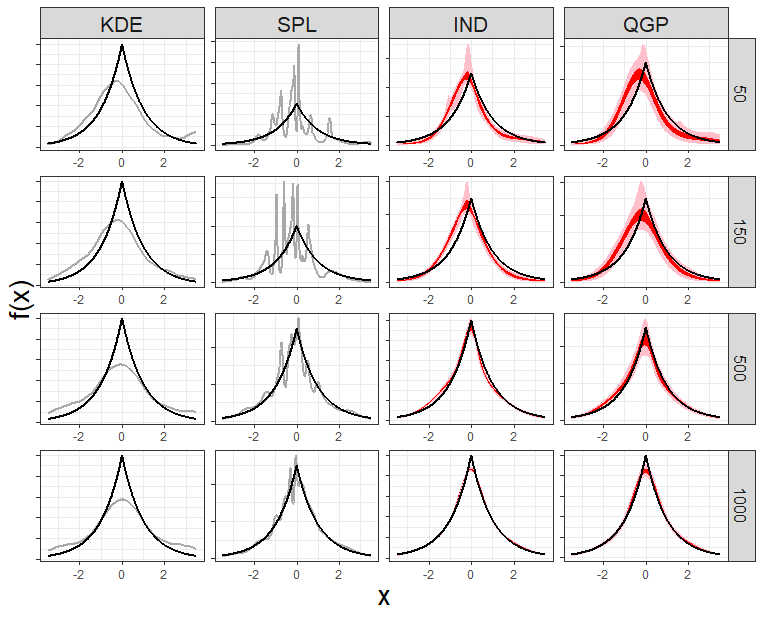
\includegraphics[width=.49\linewidth]{Images/dens_lp.png}
  % \caption{A subfigure}
  % \label{fig:sub2}
%\end{subfigure}
\caption{QM fits of $K=23$ quantiles by KDE, SPL, IND, and QGP for $n \in \{50, 150, 500, 1{,}000\}$. The quantiles were sampled from the Laplace distribution $La(0,1)$. The quantile fits (left) show the true quantiles (black) with either the QM fit line (grey) or the credible intervals of 50\% (red) and 95\% (pink). 
The estimated PDF plots (right) show the true PDF (black) with either a the QM estimated PDF (grey) or the credible intervals of 50\% (red) and 95\% (pink).}
\label{fig:lp_fits}
\end{figure}


\begin{figure}[hbt!]
\centering
%\begin{subfigure}{.5\textwidth}
  \centering
  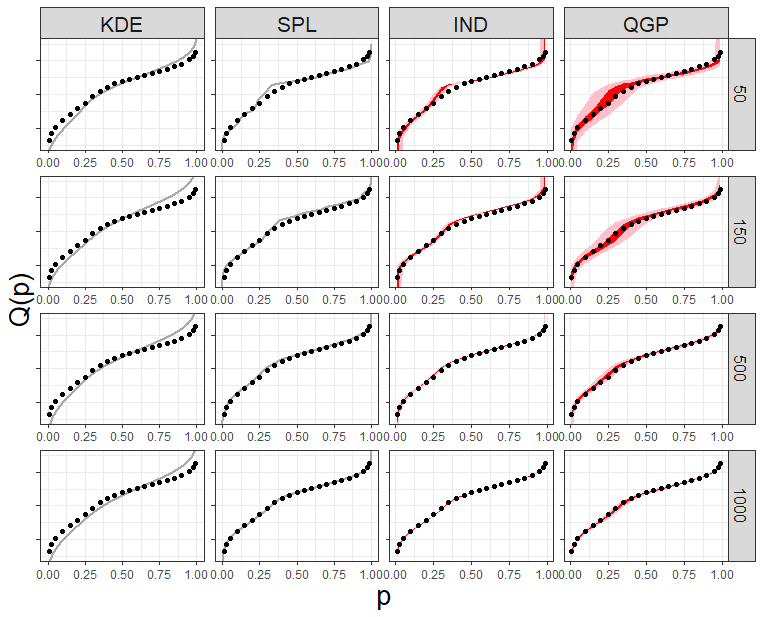
\includegraphics[width=.49\linewidth]{Images/quants_gmix.png}
  % \caption{A subfigure}
  % \label{fig:sub1}
%\end{subfigure}%
%\begin{subfigure}{.5\textwidth}
  \centering
  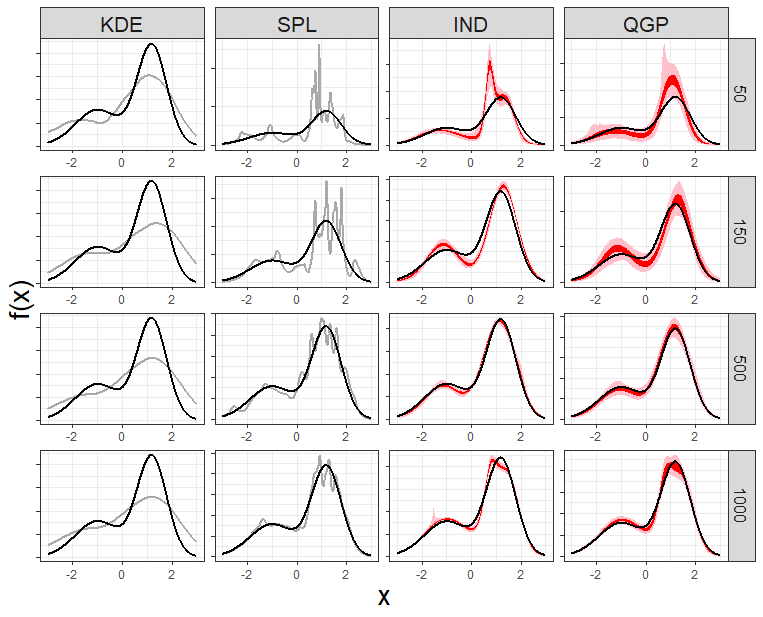
\includegraphics[width=.49\linewidth]{Images/dens_gmix.png}
  % \caption{A subfigure}
  % \label{fig:sub2}
%\end{subfigure}
\caption{QM fits of $K=23$ quantiles by KDE, SPL, IND, and QGP for $n \in \{50, 150, 500, 1{,}000\}$. The quantiles were sampled from the two component normal mixture distribution $w N(-1, 0.9) + (1-w)N(1.2, .6)$ where $w = 0.35$. The quantile fits (left) show the true quantiles (black) with either the QM fit line (grey) or the credible intervals of 50\% (red) and 95\% (pink). 
The estimated PDF plots (right) show the true PDF (black) with either a the QM estimated PDF (grey) or the credible intervals of 50\% (red) and 95\% (pink). }
\label{fig:gmix_fits}
\end{figure}



Figure \ref{fig:uk_cover} shows the simulated coverage of the true quantiles for four values of $K$ for QGP, ORD, and IND fits. The percent coverage is averaged over all $K$ quantiles and all 500 simulated replicates. The two figures show the 50\% and 95\% coverage for the three models EV, LA and MIX. The plots show that the QGP and ORD models are largely able to meet and exceed the nominal coverage where the IND model falls very short. Because it took a long time to evaluate the QF when calculating coverage, calculation was done on a thinned sample of the posterior distribution where only every $100^{th}$ HMC draw was kept so that the coverage was calculated using 6,000 posterior draws rather than the full 60,000.

\begin{figure}[hbt!]
%\begin{subfigure}{.465\linewidth}
  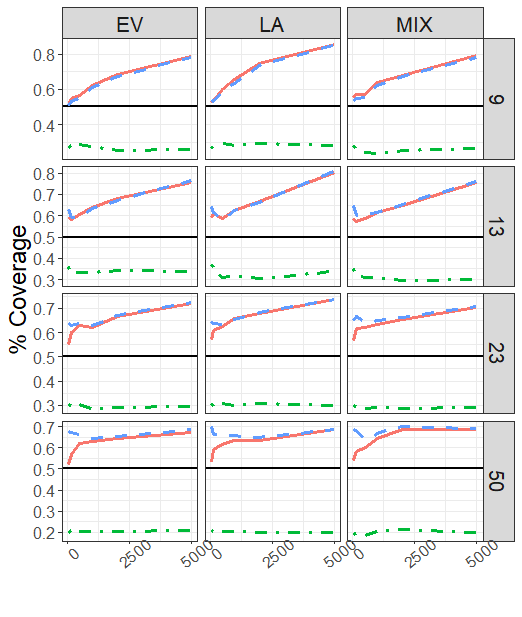
\includegraphics[width=.4\linewidth]{Images/uk_cover50.png}
  % \caption{}
  % \label{MLEDdet}
%\end{subfigure}\hfill % <-- "\hfill"
%\begin{subfigure}{.532\linewidth}
  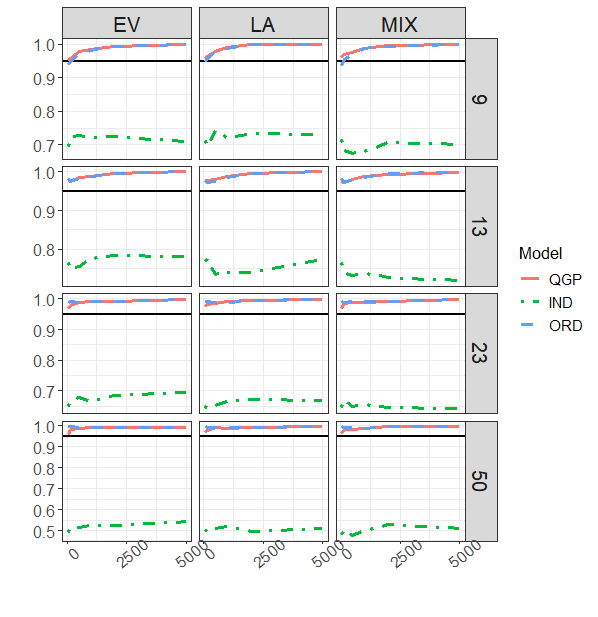
\includegraphics[width=.4\linewidth]{Images/uk_cover95.png}
  % \caption{}
  % \label{energydetPSK}
%\end{subfigure}
\caption{Percent coverage of the true quantile values for select quantiles for 500 simulated replicates of sample quantiles averaged over all quantiles. Faceted by the true EV, La, and normal mixture distributions and for $K \in \{9, 13, 23, 50\}$. The plots shows percent coverage for the 50\% credible intervals (left) and 95\% credible intervals (right). The models included are QGP, ORD, and IND. The vertical bar (black) shows the nominal coverage level.}
\label{fig:uk_cover}
\end{figure}





Figure \ref{fig:uk_dists} shows the UWD1, TV, and KLD distances between QM and true distributions averaged over 500 simulation replicates for the five QM methods. In the UWD1 plots, the SPL appears to match the true distribution only slightly better than the QGP, ORD, and IND for $K = 9$, but the difference is almost unnoticeable for larger $K$. For TV, SPL appears to perform the best except for the cases where $K \in\{23, 50\}$ where the QGP, ORD, and IND perform slightly better. There is also more separation between the performance of the QGP, ORG, and IND under TV. In most cases, the QGP and ORD perform similarly, though where the true model is a normal mixture distribution, QGP performs better. QGP and ORD both also outperform IND in a few cases. The results for KLD are similar to those for TV.

\begin{figure}[hbt!]
%\begin{subfigure}{.456\linewidth}
  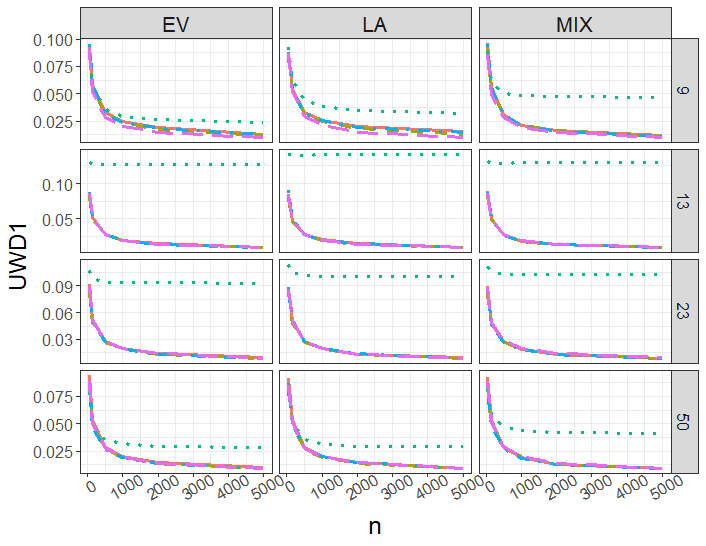
\includegraphics[width=.4\linewidth]{Images/uk_uwd1.png}
  % \caption{}
  % \label{MLEDdet}
%\end{subfigure}\hfill % <-- "\hfill"
%\begin{subfigure}{.52\linewidth}
  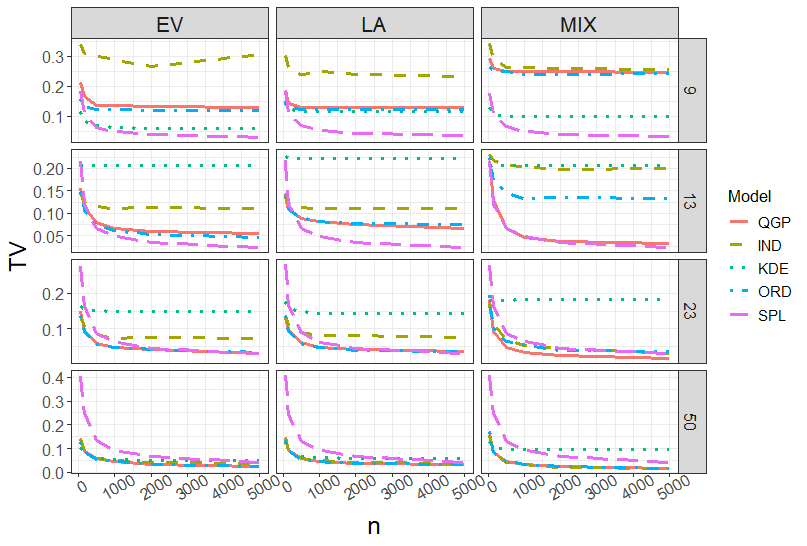
\includegraphics[width=.4\linewidth]{Images/uk_tv.png}
  % \caption{}
  % \label{energydetPSK}
%\end{subfigure}

\medskip % create some *vertical* separation between the graphs
%\begin{subfigure}{.53\linewidth}
  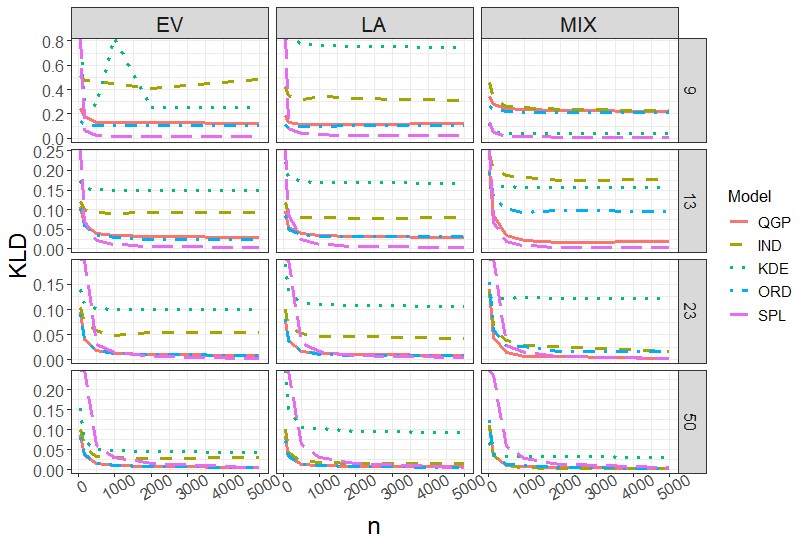
\includegraphics[width=.4\linewidth]{Images/uk_kld.png}
  % \caption{}
  % \label{velcomp}
%\end{subfigure}\hfill % <-- "\hfill"
\tiny
\caption{Distance between the true distribution and the QM estimated distribution averaged over 500 simulation replicates and measured by UWD1 (top left), TV (top right), and KLD (bottom). Plots are faceted by number of quantiles $K \in \{9, 13, 23, 50\}$ and distribution with the distributions being extreme value (EV), Laplace (LA), and two component normal mixture (MIX). Lines are colored and shaped by QM method, and are drawn by increasing sample size $n$.}
\label{fig:uk_dists}
\end{figure}




This section shows the ability of the QGP model to accurately perform parameter inference and QM when given sample quantiles. Although the inference for QGP is asymptotic, the QGP performance in inference and in QM is similar to that of ORD where the inference is exact. There are also circumstances where the QGP may outperform the ORD as shown in cases where the QF is easily evaluated but where the CDF is difficult to evaluate. Another case where the QGP outperformed the ORD was in QM of the normal mixture distribution. An advantage that the QGP has over SPL and KDE is that it provides accurate uncertainty estimation of quantile uncertainty where SPL and KDE provide no uncertainty estimation.











\section{CDC flu forecasts analysis} \label{sec:qm_analysis}


% In this section, we fit the QGP model to quantile forecasts from the 2023-24 CDC flu forecasting competition. 
% Doing this allows for tools to be used to compare forecast performance between models and build ensemble forecasts beyond what is possible using only quantile forecasts \cite[]{mathis2024evaluation,wadsworth2023mixture}.  
In this section, the QGP model is used for QM of quantile forecasts targeting US flu hospitalizations. Beginning in 2013, the CDC began hosting a yearly forecast competition of the influenza outbreak in the US. This competition is known as FluSight. The flu epidemic typically begins in the fall and ends in late spring the following year, and the forecast competition lasts around 30 weeks starting in October and ending in May. FluSight involves several academic and industry research teams who each independently develop forecasts  every week for predicting certain flu targets for future weeks \cite[]{biggerstaff2016results}. During the 2022-23 and 2023-24 seasons, the forecast targets were the 1, 2, 3, and 4-week ahead hospitalizations as reported by Health and Human Services (HHS) for the 50 US states, Puerto Rico, the District of Columbia, and the nation as a whole. The data for weekly hospitalizations of flu patients may be found at \cite{healthdata2024covidts}. The official guidelines of the most 2023-24 FluSight and all submitted quantile forecasts are publicly available at \cite{mathis2023flusight} \cite[]{mathis2024evaluation}. 



Participating teams were free to create forecasts however they pleased, but forecasts for each target were required to consist of 23 quantiles for the probability levels $\boldsymbol{p} =(0.01, 0.025, 0.5, 0.1, ..., 0.95, 0.975, 0.99)$, which were given by FluSight. Figure \ref{fig:quant_forcs_us} shows examples of quantile forecasts of the same target from 12 participating teams. Each plot shows the log forecast for hospitalizations in the US for the week of January 13, 2024, and it is clear that there are major distributional differences between forecasts.
We denote a quantile forecast for flu hospitalizations as $\hat{Q}^{(H)}(\boldsymbol{p}) = (\hat{Q}^{(H)}(0.01), ..., \hat{Q}^{(H)}(0.99))$. 
The general quantile forecast representation format allowed for forecasts to be compared by the same metric, the weighted interval score (WIS), and to be easily combined into a multi-model ensemble forecast \cite[]{mathis2024evaluation}. However, under the quantile representation, the tools for scoring forecasts and for building ensemble models are limited as many of the existing tools for scoring forecasts and constructing ensembles require CDFs or PDFs \cite[]{wadsworth2023mixture,ranjan2010combining}. Because of these limitations, it may be desirable to approximate continuous distributions from the quantile forecasts to allow for more flexibility in scoring or ensemble building. In this section, we fit the QGP model for QM to every forecast of hospitalizations submitted to the FluSight during the 2023-24 season, and an analysis is made to compare the scoring of the quantile forecasts to QGP estimated forecasts using proper scoring rules.

\begin{figure}[hbt!]
    \centering
    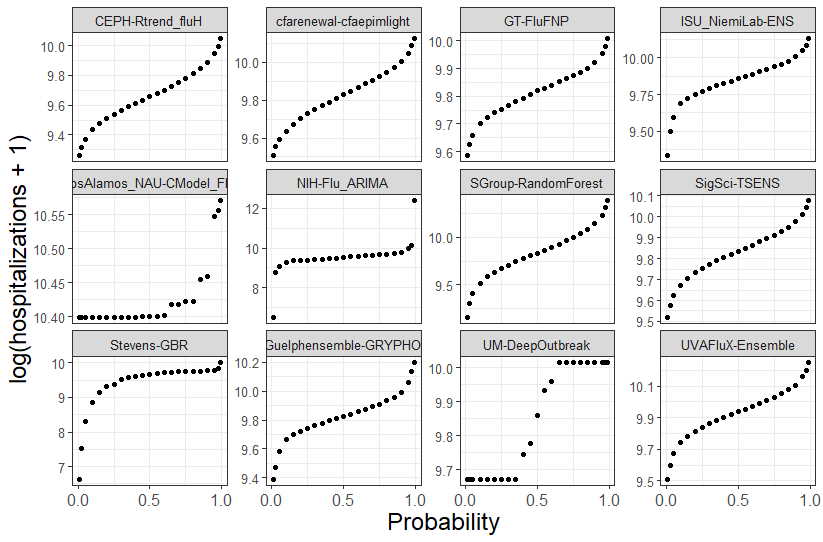
\includegraphics[scale=.6]{Images/quant_forcs_us_01_13_24.png}
    \caption{1 week ahead log flu hospitalization quantile forecasts from 12  teams who participated in the 2023-24 CDC flu forecast competition. Forecasts are for the national level during the week of January 13, 2024.}
    \label{fig:quant_forcs_us}
\end{figure}

Before fitting a QGP model to a quantile forecast we transformed the quantiles $\hat{Q}^{(H)}(\boldsymbol{p})$ to $\text{log}(\hat{Q}^{(H)}(\boldsymbol{p}) + 1)$ so that forecasts for all states were on a similar scale. The model fit was the same as the QGP fit in section \ref{sec:uk_matching}, including the same prior distribution assignments.
According to the official forecast competition rules, no forecast could include quantiles that were less than 0. As a result, there were forecasts with one or many quantiles equal to 0. When fitting the QGP model, these instances of 0 values were removed so that some forecasts had $K < 23$ quantiles. Between 39 competing forecast teams, 53 locations, 29 forecast dates, and 4 horizons, there were 180,312 quantile forecasts to which the QGP was fit. For each forecast, the WIS was calculated for the quantile forecast and the continuous ranked probability score (CRPS) was calculated over the predictive distribution of the fit QGP model.

The WIS and CRPS are both proper scoring rules, which is a class of scoring rule defined so as to keep a forecaster honest in their forecasts \cite[]{gneiting2007strictly, gneiting2014probabilistic}. 
The definition for the WIS is in (\ref{eq:wis}) and is the same as that in \cite{bracher2021evaluating}. The WIS consists of the sum of multiple intervals scores (IS), the definition of which is in (\ref{eq:is}). Here $\alpha$ is the nominal level of an interval with $l$ and $r$ being the respective lower and upper bounds of the interval. $R$ is the number of intervals in the quantile forecast, $\alpha_r$ is the nominal level for the $r^{th}$ interval, and $y^*$ is the observed value which one is attempting to forecast. 

\begin{equation}
\label{eq:wis}
        WIS_{0,R}(F, y^*) = \frac{1}{R + 1/2} \times (w_0\times |y^* - median| + \sum_{r=1}^R \{w_r \times IS_{\alpha_r}(F, y^*) \} )
\end{equation}

\begin{equation}
\label{eq:is}
        IS_{\alpha}(l,r;y^*) = (r-l) + \frac{2}{\alpha}(l - y^*)\vmathbb{1}\{y^* < l\} + \frac{2}{\alpha}(y^* - r) \vmathbb{1}\{y^* > r\}
\end{equation}

% A proper scoring rule is metric which is a function of a probabilistic forecast and the realization of the event the forecast aimed to predict. A proper scoring rule is defined such that a forecaster has no incentive to present any forecast other than the one they believe is the best (see \cite{gneiting2007strictly} for details).
The CRPS is a widely used scoring rule for forecasting and is a function of the CDF of a continuous distribution thus making it unavailable for scoring quantile functions. The CRPS is defined in (\ref{eq:crps}) where $F$ is the CDF of a forecast and $y^*$ is the observed event one attempts to forecast. The definition is the same as in \cite{gneiting2014probabilistic}. 
\begin{equation}
    \label{eq:crps}
    \text{CRPS}(F, y^*) = \int_{-\infty}^{\infty} (F(x) - \vmathbb{1} (y^* \leq x))^2 dx
\end{equation}
Fitting continuous distributions to the quantile forecasts would allow for forecast comparison using the CRPS. The CRPS assesses a forecast across an entire distribution, including the tails, which the WIS is unable to do, giving more reason why one may want to perform QM on a quantile forecast. 
% Additionally, having continuous distribution forecasts allows for using many methods to build ensemble forecasts \cite[]{ranjan2010combining} which cannot be used for quantile forecasts. 
We fit the QGP model in (\ref{eq:pit_qgp}) to the forecast competition forecasts from the 2023-24 season and compare the results of scoring the given quantile forecasts by the WIS and the CRPS calculated from the posterior predictive of the QGP model. Posterior predictive samples from the QM forecasts allow for approximate calculation of the CRPS. 
To calculate the WIS, we use the \texttt{evalcast} \texttt{R} package \cite[]{mcdonald2023evalcast}, and to calculate the CRPS we use the \texttt{scoringutils} package \cite[]{jordan2019scoringutils}.

% \begin{equation}
%     \label{eq:logs}
%     \text{LogS}(f, y) = -\text{log}(f(y))
% \end{equation}
 

Figures \ref{fig:flu_horizon_corr} and \ref{fig:flu_rank_corr} show results of comparing the WIS from quantile forecasts and the CRPS from the QGP fitted forecasts. Figure \ref{fig:flu_horizon_corr} has in the $x$-axis the WIS and CRPS is in the $y$-axis. Each point is for one forecast for any participating team, season week, and state. The plot is faceted by horizon. Clearly the relationship between the quantile forecasts and the QGP forecasts are very close with high correlation near 0.9 for each horizon. 



\begin{figure}[hbt!]
    \centering
    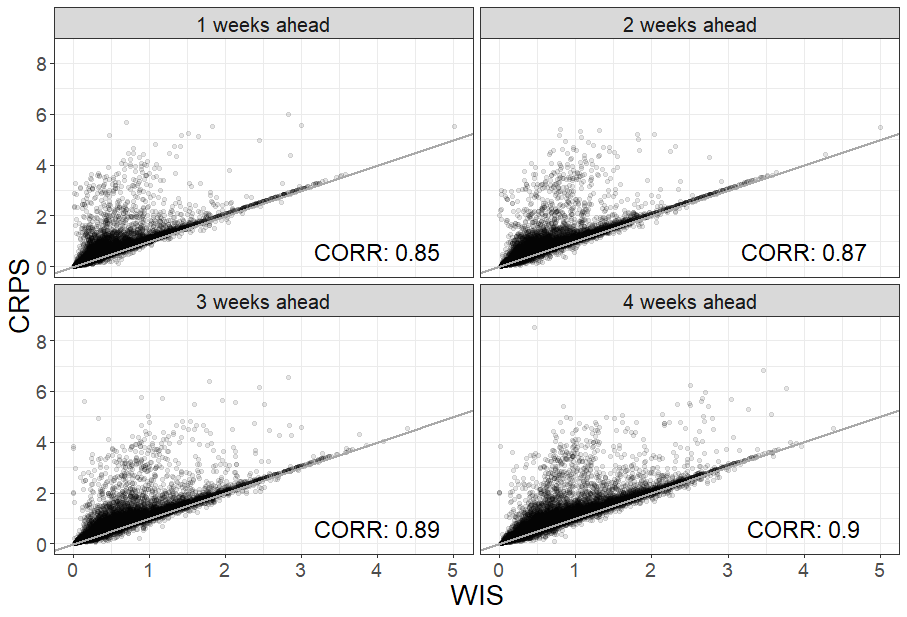
\includegraphics[scale=.5]{Images/flu_horizon_corr.png}
    \caption{Scatterplots of WIS and CRPS values for forecasts from 39 different teams for 2023-24 CDC flu forecast competition. The plots are faceted by forecast horizon. Each point represents scores for a flu forecast for one week during the season, one state, and one competing team. Points are transparent to show where more scores tended to be. Overall linear correlation is also given in the corner of each plot.}
    \label{fig:flu_horizon_corr}
\end{figure}

Figure \ref{fig:flu_rank_corr} shows the ranking of teams under the quantile forecasts' WIS vs. the QGP forecasts' CRPS. Here we say a team is considered the best performing by having the lowest score averaged across all season weeks, states, and horizons. The $x$-axis indicates where one of the 39 teams ranks by WIS and the $y$-axis where they rank by CRPS. If a block is on the diagonal line, the team's ranking was the same under the WIS as under the CRPS. The darkness of the block indicates how correlated that team's WIS is to the CRPS over the whole season. Of the 39 teams represented, 16 have the same ranking for both scores, and for over half of all teams the ranking difference between WIS and CRPS is within 3 positions. For most teams the linear correlation between WIS and CRPS is very high with only five teams having a correlation below 0.85.

\begin{figure}[hbt!]
    \centering
    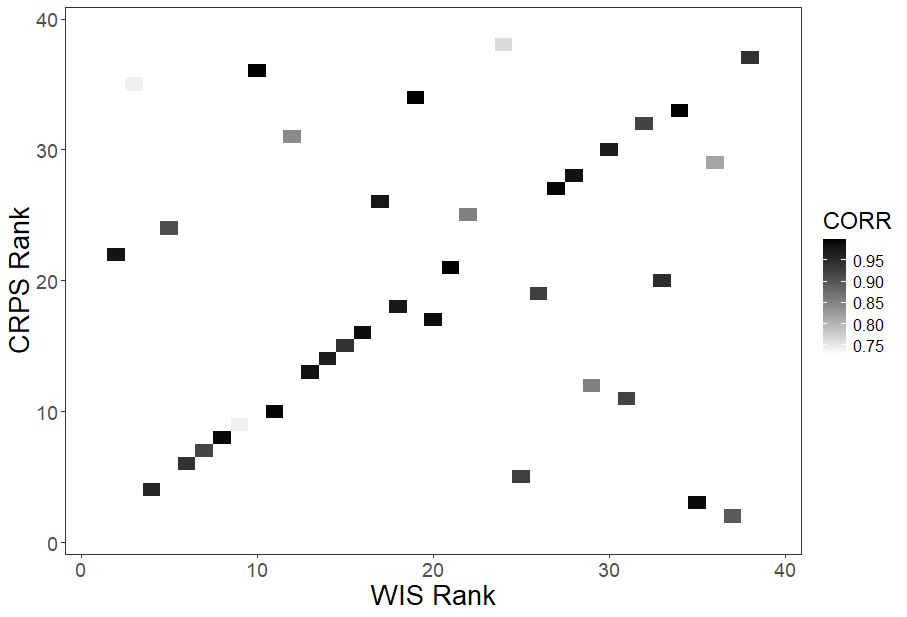
\includegraphics[scale=.45]{Images/flu_rank_corr.png}
    \caption{Blocks showing the overall season ranking of 39 competing forecast teams for WIS ($x$-axis) and CRPS ($y$-axis). Blocks on the diagonal line have the same ranking under both scores. Blocks are shaded to show correlation between WIS and CRPS for all forecasts submitted by that team.}
    \label{fig:flu_rank_corr}
\end{figure}

The results in this section show the close relationship between the quantile forecasts of the CDC flu forecast competition and the more complete forecast distributions estimated via QGP. The implications of these results include  being able to score forecasts according to scoring rules used for continuous distributions, including more problem specific rules, and being able to combine forecasts into an ensemble according to sums of CDFs or PDFs. Increased flexibility in scoring and ensemble construction could lead to improved decision making as problem specific evaluation becomes more accessible. 


%%%%
% Reference section comes before the appendix

%\bibliographystyle{acm} % use for numbered citations along with options given in preamble. Look at the main thesis.tex file

\section{Conclusion} \label{sec:qm_conclusion}

In this paper we consider the situation where quantiles with known probability levels are given as data or is given to represent a distribution rather than raw data or a fully defined distribution. We review basic properties of QFs, sample quantiles, and resulting CLTs which motivate a new model, the QGP model, for matching a set of quantiles to a continuous distribution. The QGP model is assessed for parameter estimation and inference, distribution approximation, and it is compared with other QM methods found in the literature. The simulation studies show that the QGP model does well in estimating parameters and allows for accurate measurement of uncertainty. It provides a way to perform QM for distributions defined by CDFs as well as quantile distributions where the CDF is difficult to evaluate.
An application of the QGP for QM of quantile forecasts from the 2023-24 FluSight project shows how QGP matched distributions are closely related to the original quantile forecasts in terms forecast performance among competing models. QGP forecasts, however, may be scored using a variety of scoring rules unavailable to quantile forecasts, and independent forecasts may be combined using methods made only for combining distributions by CDF or PDF functions. QGP has already been applied in chapter 4 of \cite{wadsworth2024quantile} who used the QGP predictive distributions fit in section \ref{sec:qm_analysis} to construct ensemble forecasts.

Approximating continuous distributions given only a set of estimated quantiles is not a new idea, but QGP provides a method of doing so while also accurately accounting for asymptotic uncertainty in estimated or predicted quantiles. The CLTs in this paper are limited to the case where the quantiles are estimated given a distribution sample, however similar results have been shown for the quantile regression case where quantiles are estimated in the presence of covariates \cite[]{kocherginsky2005practical, koenker1978regression}. These results could lead to additional QM modeling using the QGP model where covariates are given, and this may be more akin to the QM done by \cite{sgouropoulos2015matching}. 
Additional research for the QGP model may be in how the required distribution function is selected. Where a true model is unknown, we elected to model a distribution as a normal mixture distribution. Of course this has its limits, and using other non parametric functions, similar to \cite{gasthaus2019probabilistic}, may provide needed flexibility. As long as the selected function is continuous and once differentiable, the theory herein applies. 

The application in this paper suggests QM being useful for forecast hubs.  \cite{gerding2023evaluating} found QM a necessity in order to evaluate forecasts by a new scoring rule with COVID-19 specific applications. The extra work that comes with QM may or may not be worth the effort for any given forecast hub, but in some contexts it is something worth considering.


\section{Acknowledgments}
This work is partially supported by the National Science Foundation under Grant No. 2152117. Any opinions, findings, and conclusions or recommendations expressed in this material are those of the author(s) and do not necessarily reflect the views of the National Science Foundation.

%% The Appendices part is started with the command \appendix;
%% appendix sections are then done as normal sections
\appendix
\section{Example Appendix Section}
\label{app1}

Appendix text.

%% For citations use: 
%%       \citet{<label>} ==> Lamport (1994)
%%       \citep{<label>} ==> (Lamport, 1994)
%%
% Example citation, See \citet{lamport94}.

%% If you have bib database file and want bibtex to generate the
%% bibitems, please use
%%
\bibliographystyle{elsarticle-harv}
\bibliography{master_bib}

%% else use the following coding to input the bibitems directly in the
%% TeX file.

%% Refer following link for more details about bibliography and citations.
%% https://en.wikibooks.org/wiki/LaTeX/Bibliography_Management

% \begin{thebibliography}{00}
% 
% %% For authoryear reference style
% %% \bibitem[Author(year)]{label}
% %% Text of bibliographic item
% 
% \bibitem[Lamport(1994)]{lamport94}
%   Leslie Lamport,
%   \textit{\LaTeX: a document preparation system},
%   Addison Wesley, Massachusetts,
%   2nd edition,
%   1994.
% 
% \end{thebibliography}
\end{document}

\endinput
%%
%% End of file `elsarticle-template-harv.tex'.


